\documentclass[../main]{subfiles}
\ifSubfilesClassLoaded{
    \dominitoc
    \tableofcontentsfile
	\pagenumbering{arabic}
    \setcounter{page}{1}
	\setcounter{chapter}{6}
	\addbibresource{../Biblio/biblio.bib}
}{}

\begin{document}
\graphicspath{{../06b-Analyse-2D}, {06b-Analyse-2D}}

\chapter{Extension aux cartes en deux dimensions}\label{chap:analyse2D}

\minitoc

\section{Introduction}

Dans les chapitres précédents, nous avons étudié les propriétés d'organisation de cartes en une dimension d'une architecture de cartes CxSOM.
L'étude des cartes en une dimension nous offrait un cadre de représentation facile pour la mise en valeur des mécanismes.
Cependant, les cartes auto-organisatrices utilisées en pratique sont des cartes en deux dimensions. 
Elles apportent en effet une meilleure qualité de quantification vectorielle sur des données de plus grande dimension, tout en restant peu coûteuses en calcul.
Nous cherchons à vérifier dans ce chapitre si les mécanismes d'organisation observés sur des architectures de cartes en une dimension s'observent également sur des cartes en deux dimensions.

Le modèle CxSOM tel que présenté au chapitre~\ref{chap:modele} est adapté aux cartes de dimension et de voisinage quelconque. Les expériences présentées dans ce chapitre ne nécessitent donc pas d'adaptation de l'algorithme.
Cependant, on observe que le passage des cartes 1D aux cartes 2D classiques pose des défis supplémentaires en terme d'organisation et de convergence des poids. 
Nous avons étudié des architectures de deux et trois cartes 1D~; nous nous intéresserons dans ce chapitre à des architectures de deux et trois cartes 2D.
Le but est de vérifier si les mécanismes observés dans ces architectures de cartes 1D sont observés en 2D. 
Nous observerons en particulier les propriétés suivantes, qui sont des marqueurs d'un apprentissage associatif entre cartes~:
\begin{itemize}
	\item Les poids externes de chaque carte de l'architecture permettent une bonne quantification vectorielle de l'entrée externe
	\item Les poids contextuels définissent des zones, et se déplient sur des sous-cartes d'une carte.
	\item Les BMUs d'une carte encodent à la fois l'entrée externe et la valeur du modèle $U$.
	\item La relaxation converge en fin d'apprentissage
	\item Une carte ne recevant pas d'entrée externe est capable de générer une bonne prédiction de la modalité manquante dans l'architecture
\end{itemize}

Les exemples que nous étudions dans ce chapitre nous permettront d'identifier des limites et perspectives pour le passage des cartes 1D à 2D dans des architectures de cartes CxSOM.

\section{Présentation de l'expérience}

\subsection{Modèle d'entrées}

Jusqu'à présent, les modalités observées étaient chacune en une dimension et $U$, la variable latente également 1D.
Afin de complexifier la structure des entrées, nous choisissons cette fois d'étudier des données dont chaque modalité est en deux dimensions, et dont le modèle latent $U$ est également 2D.
Nous analyserons des architectures de deux et trois cartes, ainsi nous choisissons des modèles d'entrées de dimension totale 4 et 6.
Le modèle 4D est présenté en figure~\ref{fig:sphere_inputs}.
La variable $U$ en deux dimensions paramètre les points placés sur une sphère 3D. Les deux dimensions de $U$ sont les angles paramétrant la représentation polaire de la sphère, $\theta$ et $\phi$~; sur les représentations, nous les normalisons entre $0$ et $1$.
Pour générer les entrées, nous tirons $U$ dans $[0,1]^2$, ce qui correspond à un point sur la sphère.
Nous effectuons ensuite une rotation en 4D afin que les coordonnées du point soient distribués sur les 4 axes de la base. Cette représentation en 4D de la sphère permet de définir deux modalités en deux dimensions $\inpx\m{1}$ et $\inpx\m{2}$. Sur la figure, les points sont colorés par rapport à la valeur de $U$, ce qui correspond à la figure de gauche. 
Par symétrie, l'agencement des coordonnées importe peu. Les paires $\inpx\m{1}, \inpx\m{2}$ correspondant à un même point sont présentées lors de la même itération à l'architecture.
Plusieurs valeurs de $U$ correspondent à une même valeur de $\inpx\m{1}$, ce qui est marqué par l'existence de plusieurs couleurs de points à une même position. La même chose est observée sur $M\m{2}$.
Nous sommes donc dans un cas similaire aux tracés en une dimension, et nous chercherons à vérifier si les cartes $M\m\{1}$ et $M\m{2}$ apprennent à différencier les valeurs de $U$ par la position de leur BMU.

\begin{figure}
	\includegraphics[width=\textwidth]{sphere_inputs_colormap.pdf}
	\caption{Transformation d'une surface d'un espace 3D, paramétrée par $U$ vers un espace 4D. Les points sont positionnés sur une surface et plongés dans un espace de plus grande dimension. La rotation permet de répartir les coordonnées des points sur les quatre dimensions sans modifier la structure des entrées. Les modalités considérées sont des valeurs 2D $\inpx\m{1}$ et $\inpx\m{2}$.
	La couleur de chaque point des figures fait référence à la valeur de $U$ correspondante, dont la disposition est présentée figure de gauche. Plusieurs valeurs de $U$ différentes permettent de générer une même valeur de $\inpx\m{1}$. Par exemple, $\inpx\m{1} = (0.5, 0.7)$ correspond à $U$ autour de $(0.6,0.3)$ (vert) ou $U$ autour de $ (0.6,0.8)$ (violet).
	\label{fig:sphere_inputs}}
\end{figure}

\subsection{Architecture}

L'architecture de cartes en deux dimensions est construite sur le même principe qu'une architecture de cartes 1D, le modèle présenté au chapitre \ref{chap:modele} étant valable pour n'importe quelle dimension de carte.
Nous nous intéressons d'abord à une architecture de deux cartes. Les n\oe{}uds sont positionnées sur une grille carrée et indexés entre 0 et 1 sur chaque dimension, que nous noterons $\mathbf{p}\m{i} = (p\m{i}_0, p\m{i}_1)$ sur les figures. 
Chaque carte possède donc une couche de poids externes $\w\ext \in [0,1]^2$ et une couche de poids contextuels $\w_c \in [0,1]^2$.
Les poids contextuels représentent les positions des BMUs de l'autres cartes qui sont les positions $\mathbf{p}\m{2}$ pour la carte $M\m{1}$ et $\mathbf{p\m{1}}$ pour la carte $M\m{2}$. Nous prenons des cartes de taille $100 \times 100$.
Les activités $a_e$ et $a_c$ sont calculées par une activation gaussienne, qui est la même qu'en dimension 1.
$$a_e(\inpx,\mathbf{p}) = \exp(\frac{||\inpx - \w_e(\mathbf{p}) ||^2}{2\sigma^2})$$
de même pour $a_c$.
La norme utilisée est ici la norme euclidienne, que ce soit dans l'espace d'entrée et dans l'espace des positions de la carte.
Les fonctions de voisinage sont également définies à partir de la norme euclidienne dans l'espace des positions d'une carte.

La notion d'organisation dans une carte 2D est plus difficile à formuler que dans une carte en une dimension. 
Par exemple, la topologie intuitive d'une carte "organisée" sur le carré $[0,1]^2$ est que les quatre coins de la carte viennent se placer dans les coins du carré.
Cependant, les mécanismes d'organisation peuvent conduire à une carte tordue en son milieu, par exemple en \label{fig:torsion}. 
Cette organisation respecte la continuité des poids au sens des cartes auto-organisatrices~: deux poids proches dans la carte correspondent à des entrées proches, peut-être une configuration stable des poids, mais n'est pas forcément la topographie représentant le mieux l'espace d'entrée. 
De plus, l'organisation et la convergence des poids externes n'est pas assurée pour un rayon de voisinage constant, même dans une carte de Kohonen classique. Des travaux ont prouvé la convergence des SOM en une dimension mais seulement partiellement pour les cartes en deux dimensions, même avec des paramètres d'apprentissage décroissant \cite{flanagan_self-organisation_1996}. En pratique, la convergence des poids des SOMs en deux dimensions est observée avec un rayon de voisinage décroissant, mais pas de travaux à notre connaissance n'ont étudié le comportement des SOMs 2D lorsque les rayons restent constants. La convergence des poids des cartes est un enjeu crucial en deux dimensions.
%Des mesures d'organisation existent sur des cartes en deux dimensions \cite{Polani2001MeasuresFT}.

\begin{figure}
	\centering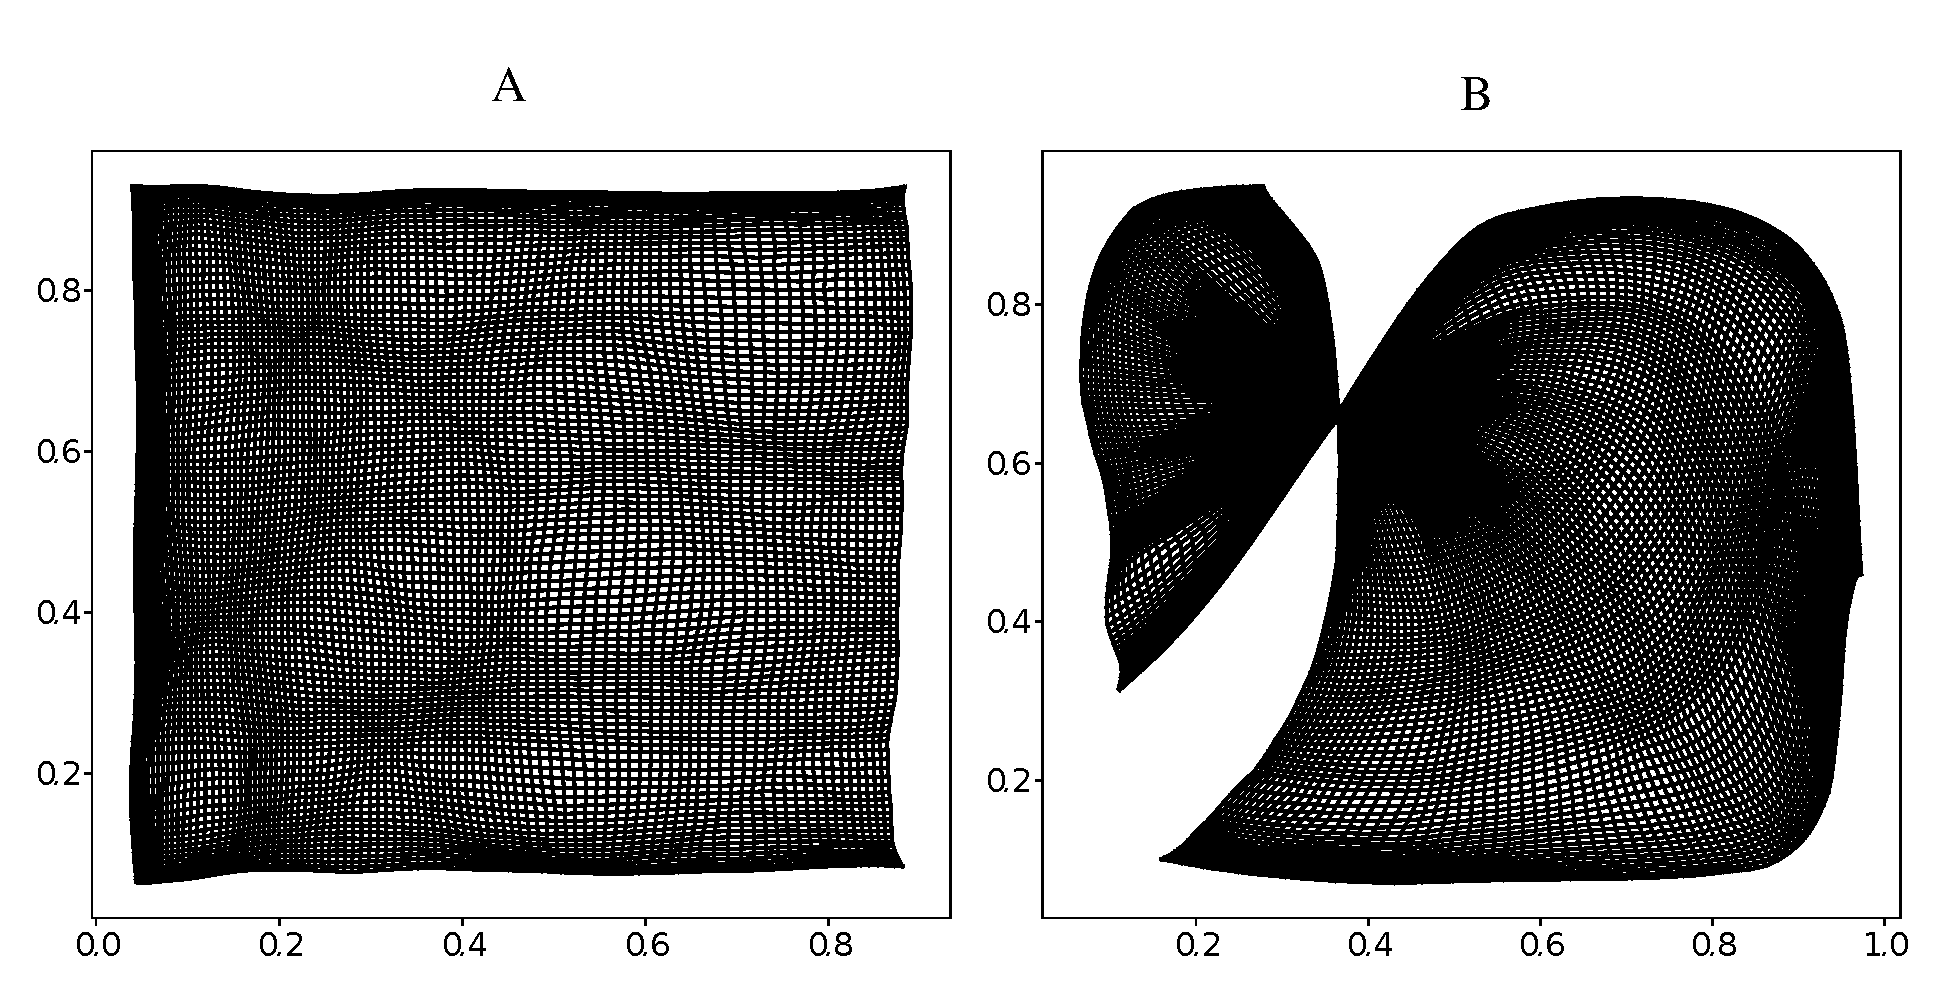
\includegraphics[width=0.7\textwidth]{we_cub_example.pdf}
	\caption{Exemple de point de torsion dans une carte 2D dépliée sur des entrées dans $[0,1]^2$ (B). La carte A au contraire est bien dépliée~: deux entrées proches sont représentées par des BMUs proches. Cette disposition présentant un point de torsion peut évoluer vers une carte bien dépliée ou vers un état stable présentant un point de torsion, en fonction des paramètres d'apprentissage. \label{fig:torsion}
	}
\end{figure}

Dans une architecture CxSOM, cela pourrait poser un problème pour l'utilisation de la position du BMU en tant que représentation de l'entrée~: deux entrées proches peuvent avoir leur BMU de chaque côté de la carte.
Dans un premier temps, nous avons choisi de favoriser le bon dépliement des poids externes en modifiant l'initialisation des poids, auparavant aléatoire. Pour cela, nous laissons les poids externes s'organiser sur 500 itérations à partir des activités externes et sans prendre en compte les poids contextuels, en prenant un grand rayon de voisinage $r_e = 0.5$. 
Ce grand rayon permet d'éviter les zones de torsion dans la carte et pré-répartit les poids externes. Après cette étape préalable, nous réduisons le rayon externe  à $r_e = 0.2$ et effectuons l'apprentissage des poids externes et contextuels comme décrit dans le modèle CxSOM. Les poids externes affinent alors leur apprentissage et les poids contextuels s'organisent sur une carte "bien dépliée".
La généralisation de l'organisation de CxSOM sur des carte "mal dépliées" sera à explorer pour assurer une robustesse de l'algorithme sur des données quelconques~: il est en effet compliqué de s'assurer du bon dépliement d'une carte en pratique sur des données de grande dimension. Nous laissons cette question à des travaux futurs.

\section{Résultats}

\subsection{Organisation des cartes sur des entrées dépendantes}

Nous étudions d'abord l'organisation des cartes sur les données prises sur la sphère 3D pivotée dans un espace en 4D décrite en figure \ref{fig:sphere_inputs}. Les données ont ici deux degrés de liberté qui sont les angles paramétrant la représentation polaire de la sphère, $U$ est ainsi en deux dimensions. 
Nous prendrons dans une première expérience les paramètres $r_c = 0.02$ et $r_e = 0.2$.
Nous nous intéressons en premier lieu à l'organisation des poids externes et contextuels des cartes. Sur des cartes 1D, nous avons observé que les poids externes s'organisent comme une carte classique, tandis que les poids contextuels forment des zones.

La figure~\ref{fig:2som_s_002_wc}, en haut, présente la disposition des poids externes et contextuels de l'architecture de deux cartes après 300 000 itérations d'apprentissage.
Nous représentons les poids externes dans l'espace des entrées~: un n\oe{}ud de la carte est positionné en $\w_e(\mathbf{p})$ qui est une position 2D.
La figure  montre que chaque carte représente ses entrées externes de la même façon qu'une carte classique, ce qui est bien attendu du modèle CxSOM. Chacune des cartes s'étend sur le disque dans lequel sont tirées leurs entrées externes.
En bas, nous représentons les poids contextuels de la carte sous forme de carte de coloration. Un pixel positionné en position $\mathbf{p}$ est coloré selon la valeur de son poids $\w_c(\mathbf{p})$, une valeur en deux dimensions.
Ces tracés font apparaître des motifs alternés dans chaque carte qui rappellent les motifs présents en une dimension. Le comportement observé en 1D se retrouve donc sur cette exemple de carte 2D.
Une première différence avec les cartes en une dimension est la forme des zones, moins régulières. Comme en une dimension, ces zones dépendent des rayons de voisinage $r_c$ et $r_e$. Nous verrons leur influence plus bas. 

\begin{figure}
	\begin{minipage}{\textwidth}
		\centering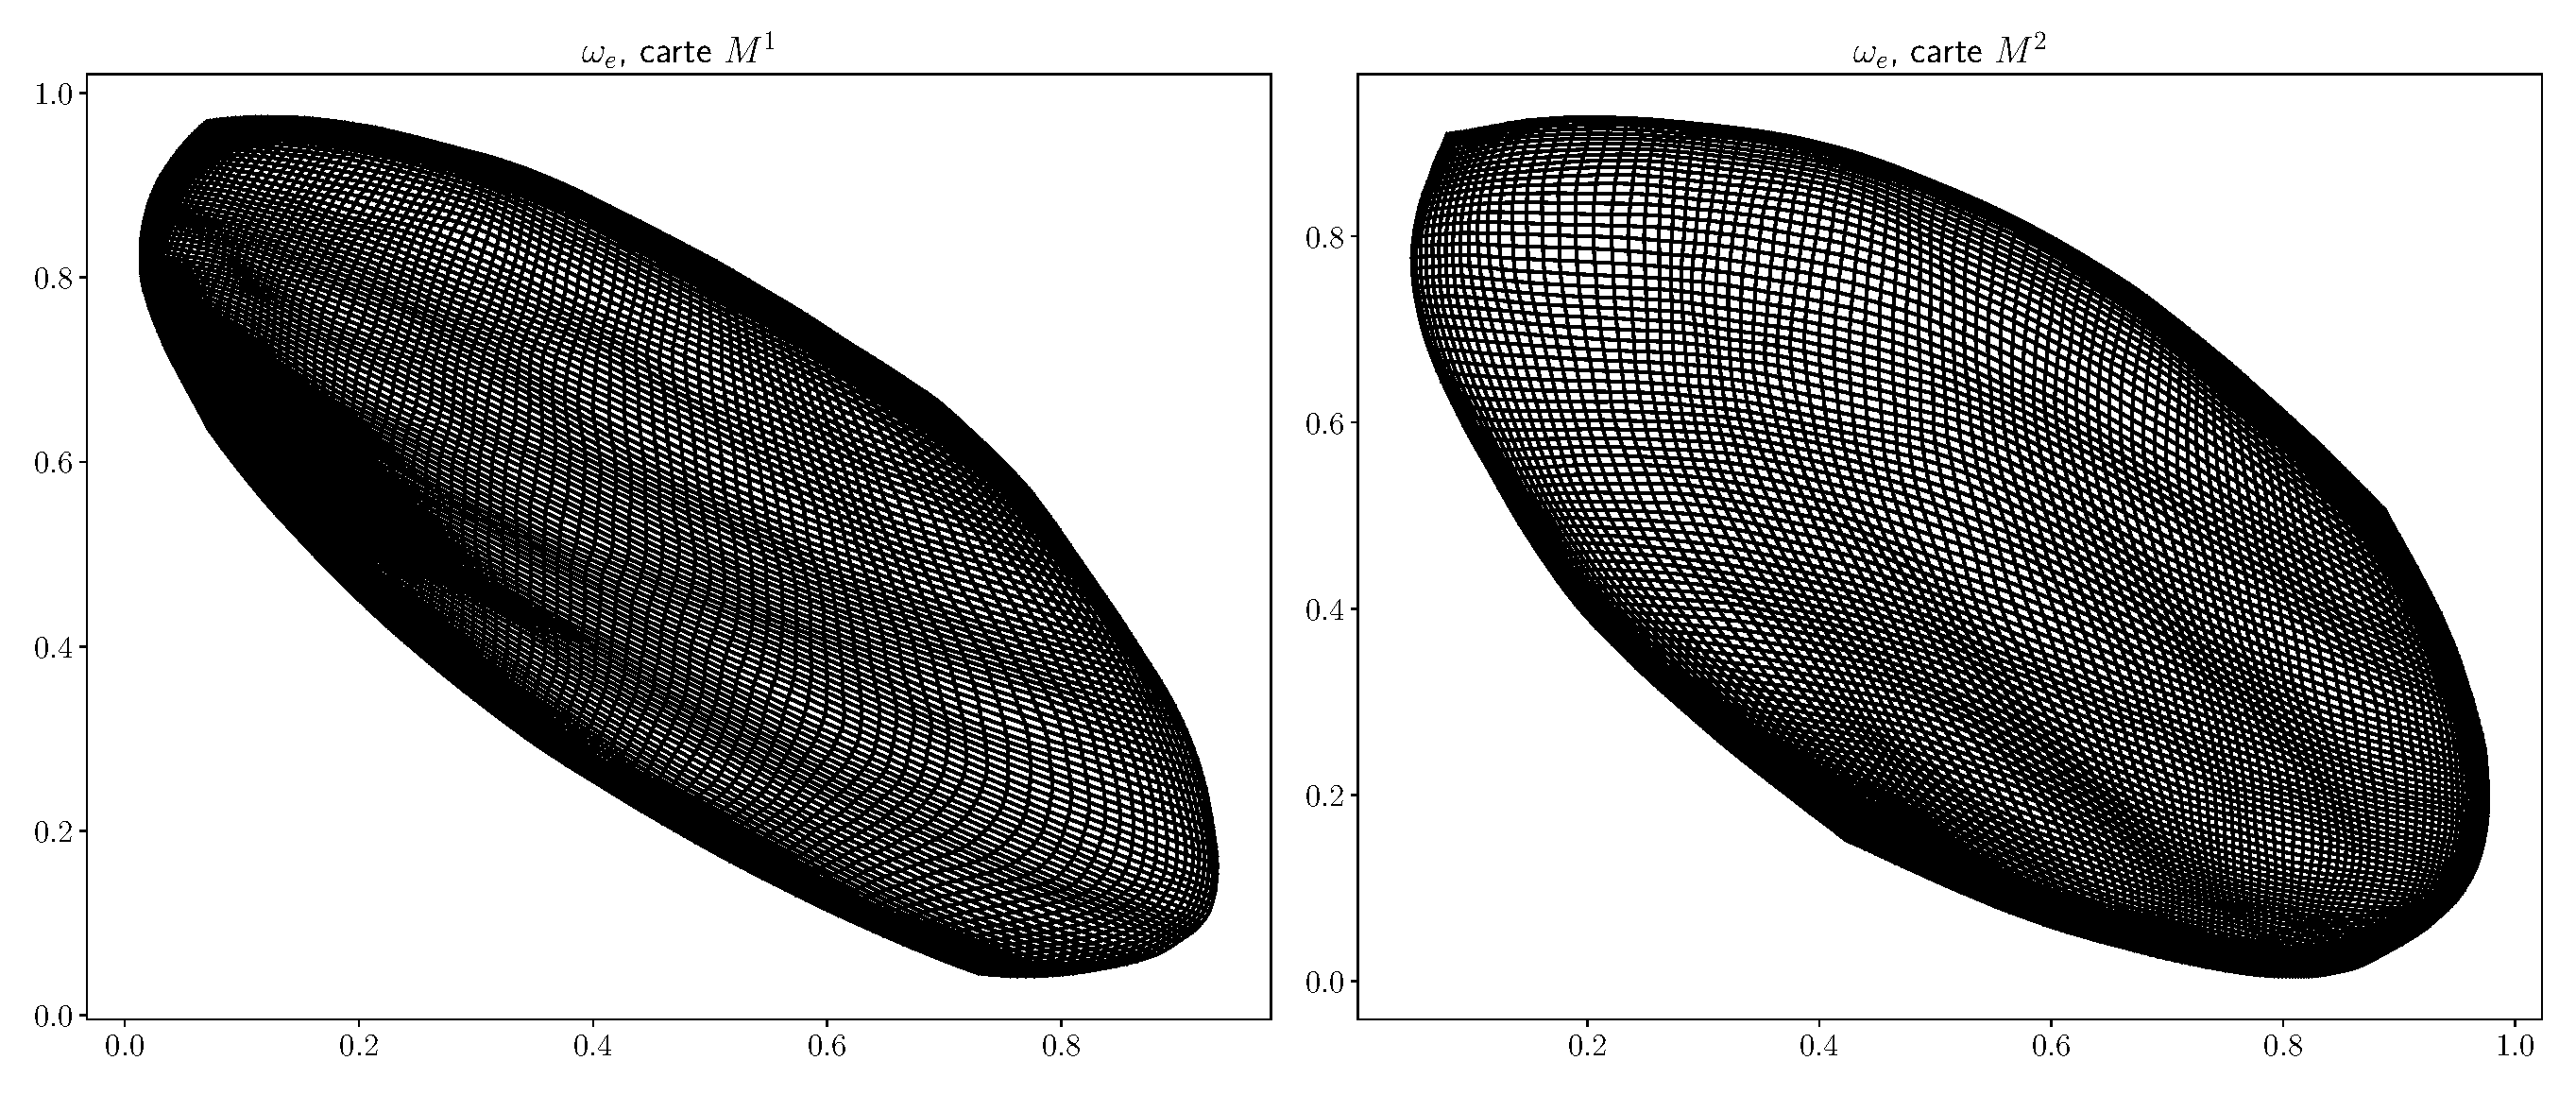
\includegraphics[width=0.8\textwidth]{we_rc002_afterbug.pdf}
	\end{minipage}
	\begin{minipage}{\textwidth}
		\centering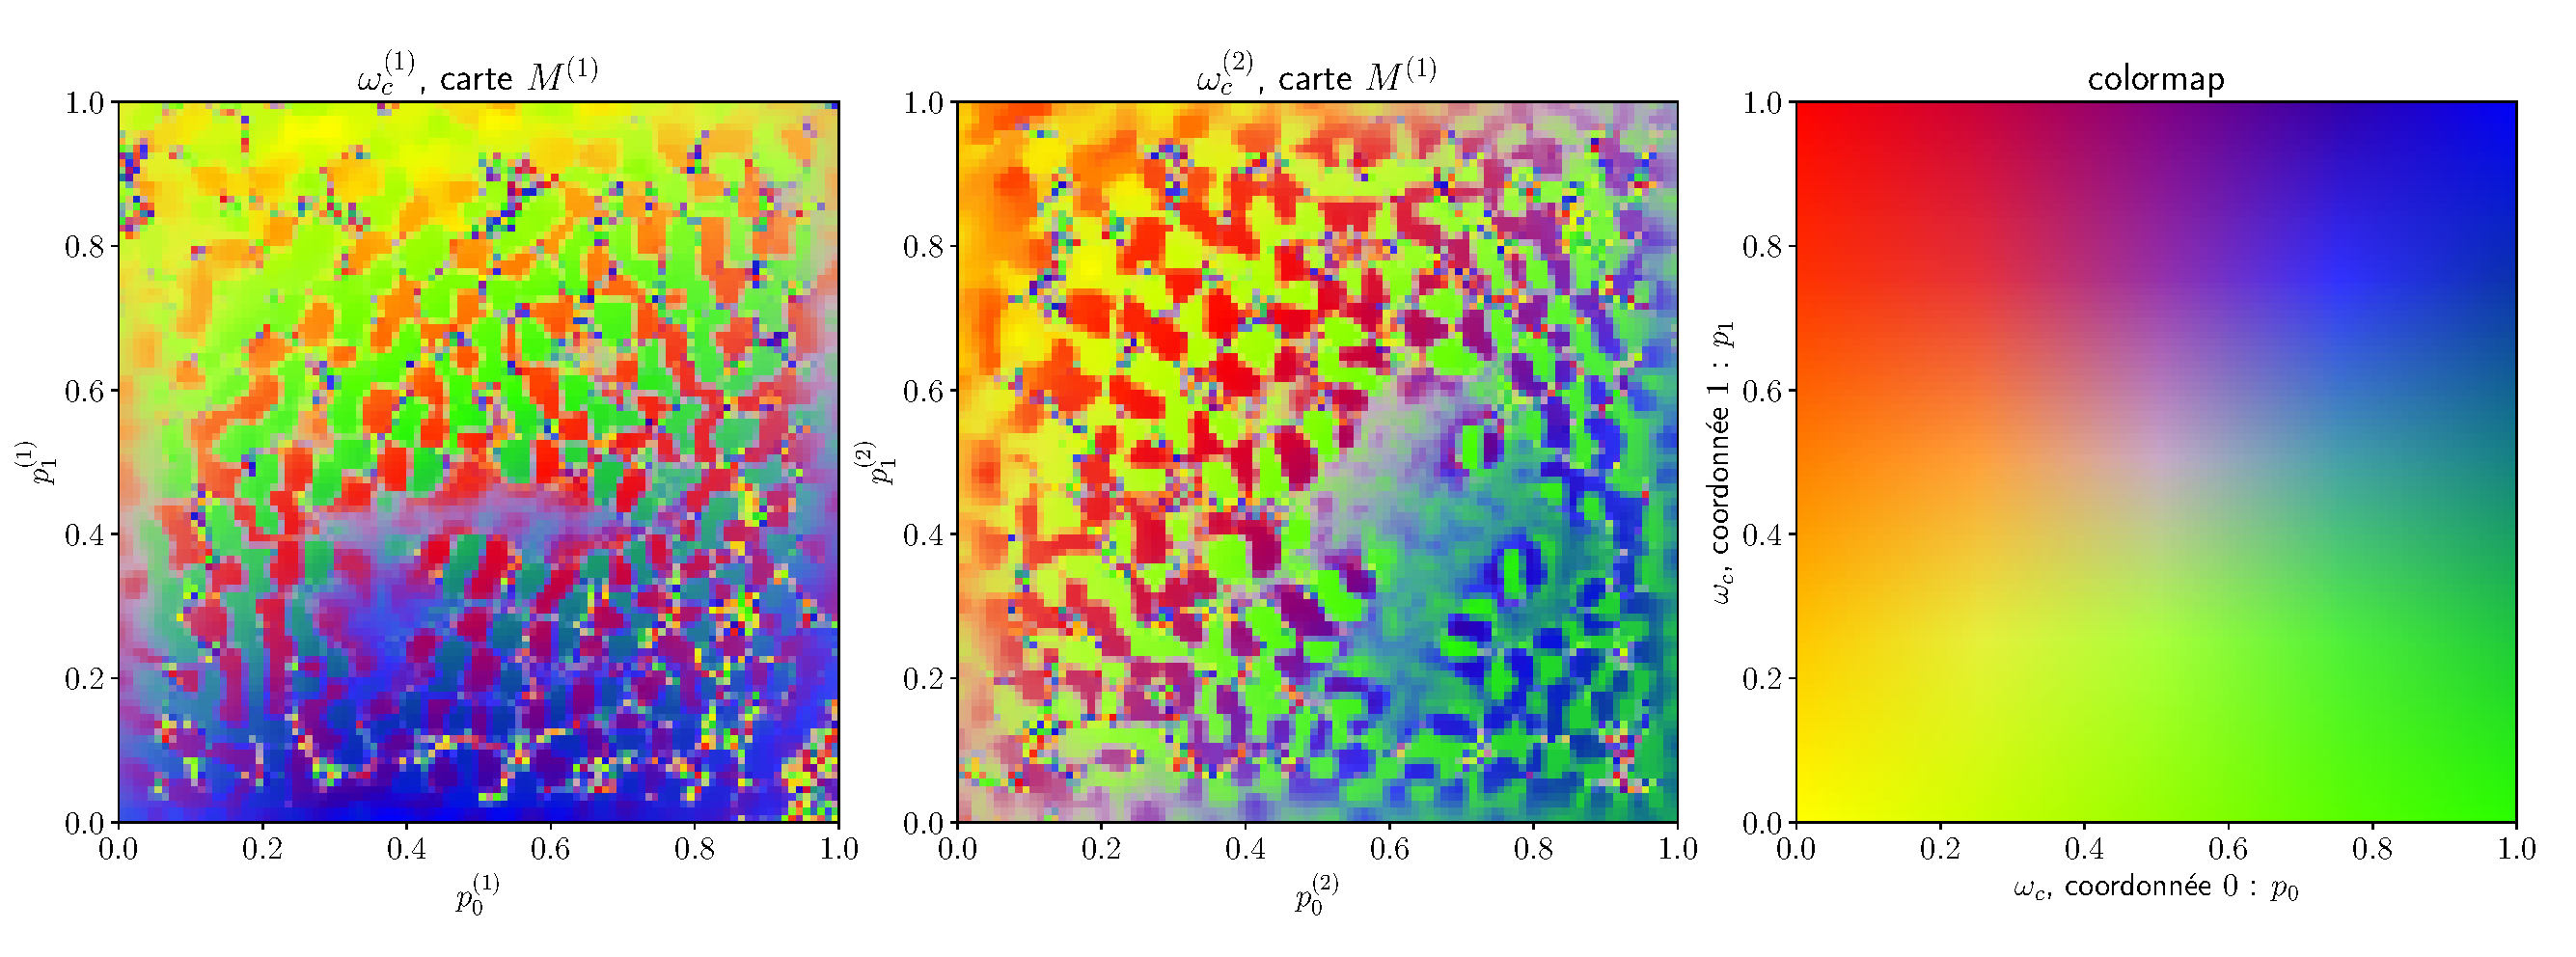
\includegraphics[width=\textwidth]{wc_rc002_afterbug_nopoints.pdf}
		\caption{Tracé des poids contextuels d'une architecture de cartes, organisées sur une sphère dans un espace 4D, avec $r_e =0.2$ et $r_c = 0.02$.
		\label{fig:2som_s_002_wc}}
	\end{minipage}
\end{figure}

Dans un deuxième temps, nous nous intéressons à l'apprentissage du modèle $U$ dans chacune des cartes. Comme en 1D, nous pouvons tracer la valeur de $U$ selon la position du BMU dans chaque carte sur une étape de test lancée sur la configuration des poids après apprentissage. Cette étape de test comporte 10000 points.
Ces tracés permettent de faire figurer les zones mortes de la carte. En une dimension, nous avons noté que les zones de BMU correspondent aux zones des poids contextuels~; deux zones proches codent pour des valeurs de $\inpx$ proches mais pour des $U$ différents. Dans chaque carte, $U$ est alors une fonction du BMU~: cette propriété marque l'apprentissage du modèle par chacune des cartes. 

La figure $\ref{fig:U_BMU}$ présente les valeurs de la variable 2D $U$, représentée par la couleur des points, en fonction de la position du BMU $\bmu\m{1}$ et $\bmu\m{2}$ de chaque carte. Nous y faisons figurer deux points en rouge et bleu~: ces deux entrées ont la même valeur de $\inpx\m{1}$ mais une valeur différente de $\inpx\m{2}$ et donc $U$.
Nous voyons sur la figure que les comportements observés en 1D se reproduisent dans cet exemple 2D. La figure fait apparaître des zones blanches, sans points~: il s'agit des zones mortes, séparant les zones de BMUs. Des BMUs proches codent pour des entrées ayant la même valeur de $\inpx$ et de $U$. Les points rouge et bleu sont au contraire envoyés dans des zones différentes, mais proches dans la carte.
Contrairement aux cartes 1D, il est difficile de voir sur les tracés si $U$ est une fonction de $\bmu$ dans chaque carte. Le ratio de corrélation est calculable sur des valeurs en deux dimensions.
Nous obtenons $\eta(U|\bmu\m{1}) = 0.99 $ et $\eta(U|\bmu\m{2}) = 0.99 $.
Ces valeurs sont de $\eta(U|\bmu\m{1}) = 0.94 $ et $\eta(U|\bmu\m{2}) = 0.98$ pour des cartes ayant appris indépendamment sur les mêmes entrées 2D.
En effet, la répartition des valeurs de $U$ selon $\inpx\m{1}$ et $\inpx\m{2}$ donne déjà des ratios de corrélation élevés~:
$\eta(U|\inpx\m{1}) = 0.91$ et $\eta(U|\inpx\m{2}) = 0.98$. 
Cet indicateur permet bien d'observer un apprentissage de $U$ par le modèle CxSOM lorsqu'on le compare à la valeur des entrées. Une meilleure analyse de l'indicateur reste à étudier pour une étude claire de données en plus grande dimension, dans laquelle un tracé n'est plus possible.

\begin{figure}
	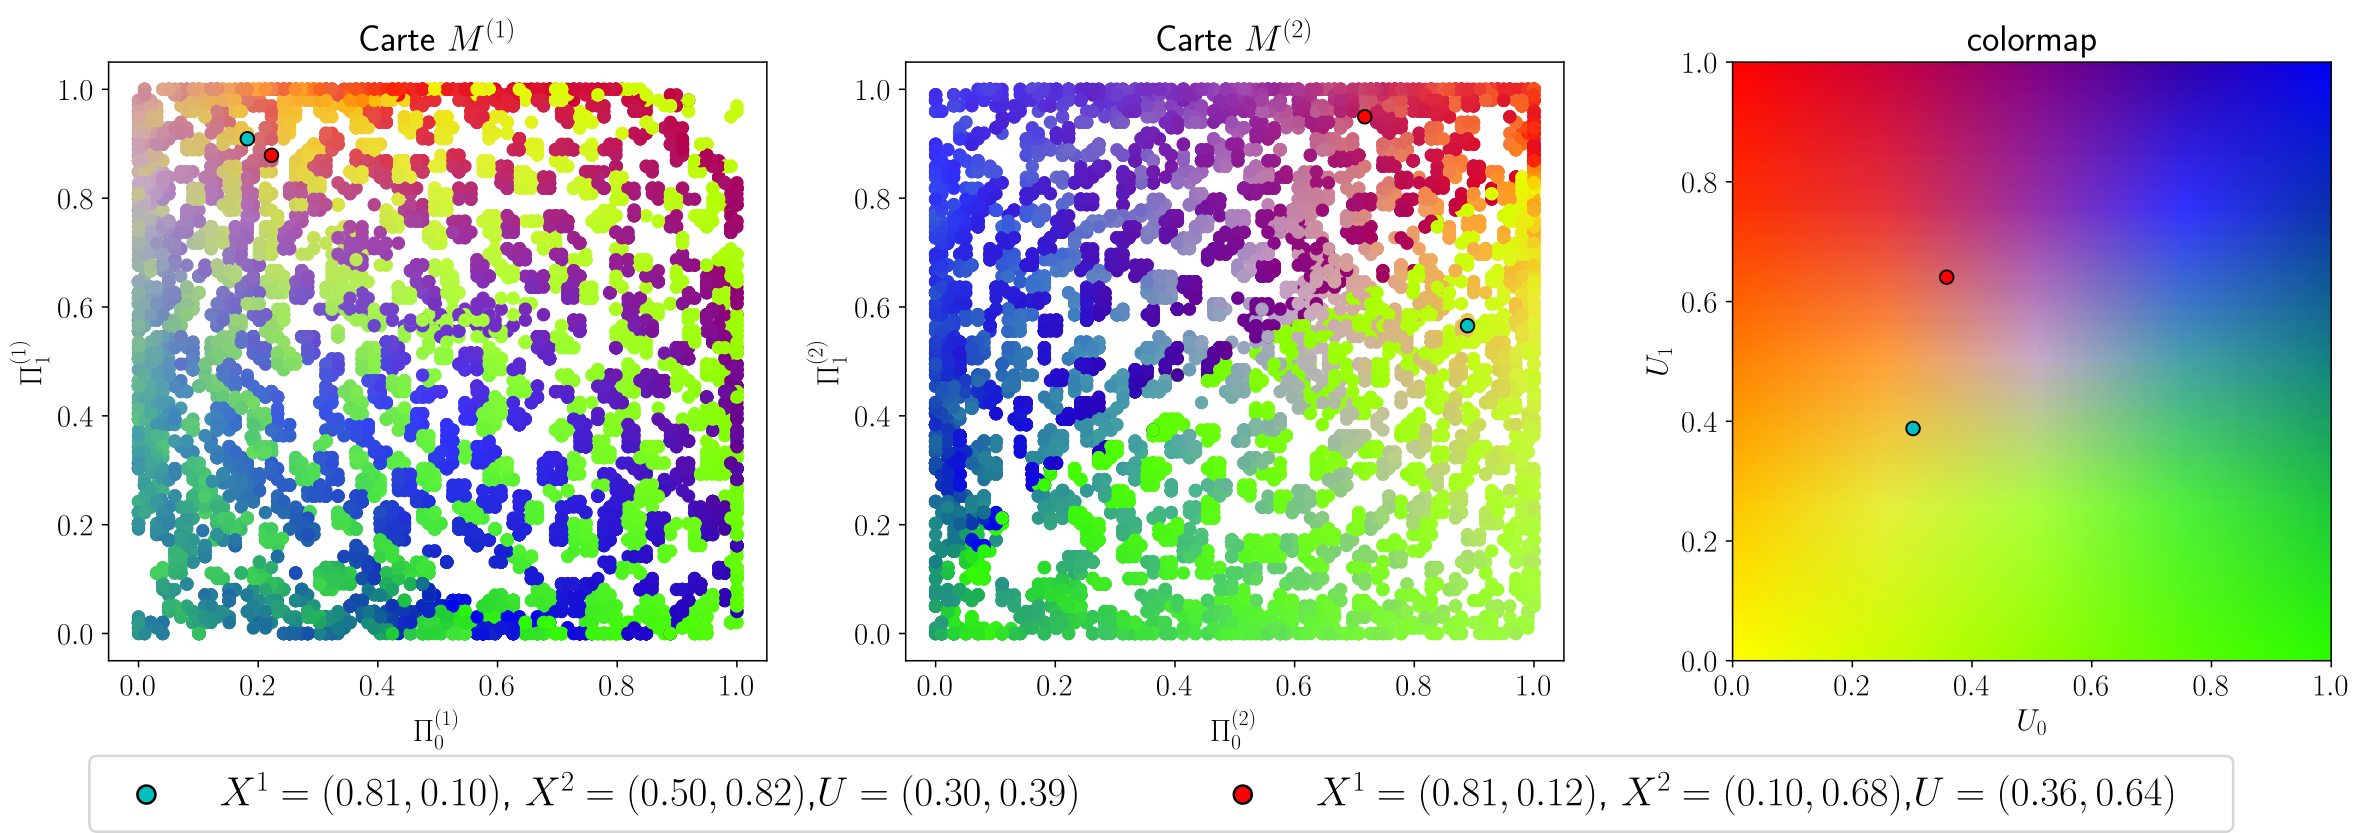
\includegraphics[width=\textwidth]{U_BMU_2SOM_2D.pdf}
	\caption{Disposition des valeurs de $U$, ici une variable en deux dimensions, selon les valeurs du BMU $\bmu$ dans chaque carte. Les tracés font apparaître que des zones de BMUs se spécialisent pour une valeur de $U$, comme ce qui était observé en une dimension. Les points mis en valeurs en rouge et bleu ont des valeurs très proches d'entrée $X\m{1}$, mais des valeurs différentes pour $U$ et donc $\inpx\m{2}$. Leurs BMUs sont séparés sur la carte $M\m{1}$ et envoyés dans des zones distinctes.
	\label{fig:U_BMU}}
\end{figure}

\begin{figure}
	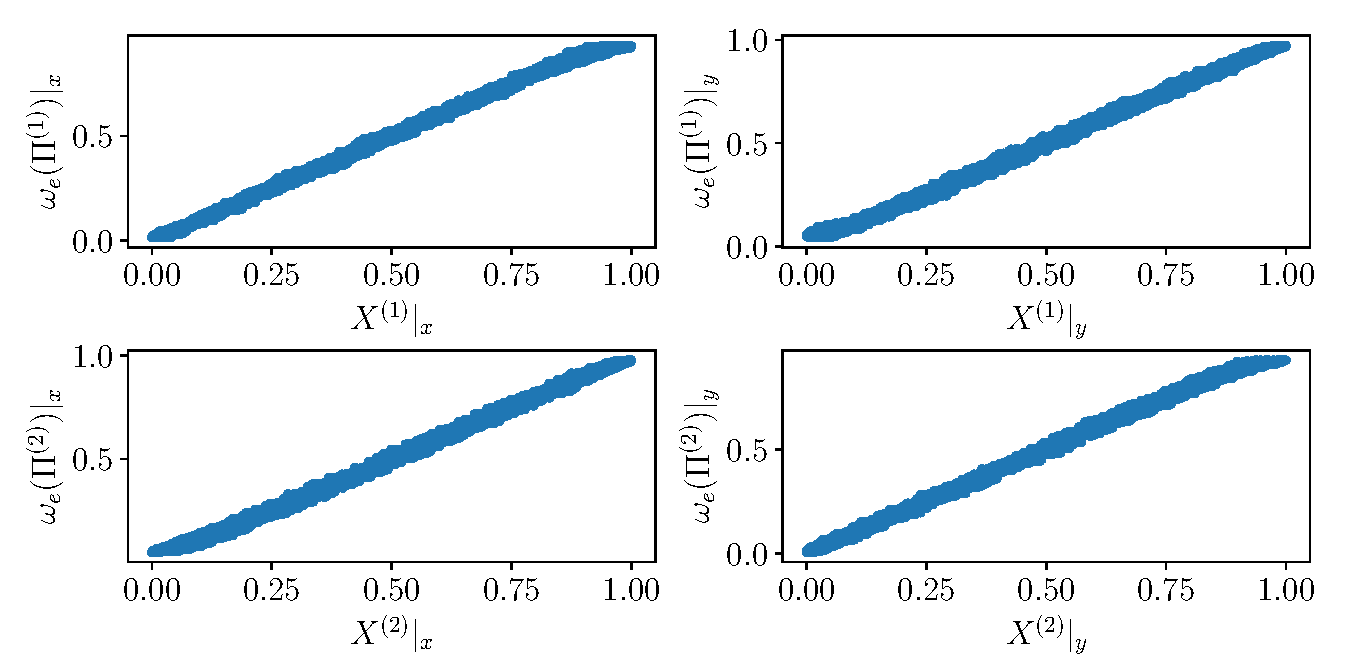
\includegraphics[width=\textwidth]{error-2SOM.pdf}
	\caption{Tracé de l'erreur de quantification vectorielle des poids externes sur l'architecture de deux cartes. Les coordonnées de chaque élément sont tracées séparément. \label{fig:qv2D}}
\end{figure}
\subsection{Convergence des poids et motifs de poids contextuels}

La formation de zones de poids contextuels dépend des paramètres de la carte et notamment  rapport entre rayon de voisinage.
Nous comparons dans cette section la forme des motifs de poids contextuels pour une même taille de $r_e$ mais des rayons de poids contextuels $r_c$ différents.
Nous nous demanderons si les poids contextuels et externes convergent dans cette disposition et dans ce cas, quels sont les motifs formés par les poids.
Les Figures~\ref{fig:rc_003}, \ref{fig:rc_005} et \ref{fig:rc_002} présentent ainsi l'évolution des poids contextuels au cours de l'apprentissage pour une même distribution de données d'entrées et $r_c = 0.05, 0.03$ et $0.02$
Nous remarquons que l'expérience avec $r_c = 0.02$ conduit à une configuration stable des poids contextuels, \ref{fig:rc_002}. Cette convergence est également observée dans l'expérience avec $r_c = 0.03$ en figure \ref{fig:rc_003}. Au contraire, les poids contextuels ne montrent pas clairement de convergence pour $r_c =0.05$~: à l'issue des 500 000 itérations, nous pouvons remarquer des changements clairs dans la structure des poids contextuels. Les poids contextuels ne forment par ailleurs pas de motifs clairement définis, au contraire des deux jeux de paramètres précédents.

Cependant, la notion d'organisation n'est pas à évacuer~: nous observons une organisation des poids contextuels similaires dans ces trois expériences. Les poids contextuels tendent en effet à s'organiser sous une forme hélicoïdale dans les trois expériences. Pour les cas où $r_c = 0.02$ et $r_c = 0.03$, cette hélice est stable à partir de 200 000 itérations, mis à part quelques zones oscillant au cours des itérations. 
Dans le cas ou $r_c = 0.05$, cette hélice évolue en tournant sur elle-même et apparaît toujours évoluer après 500 000 itérations.
La similarité existant entre la forme des poids montre que les motifs dépendent bien de la relation entre entrées, ici la sphère.

Nous pouvons conclure de ces observations préliminaires en deux dimensions que la formation de zones est un mécanisme qu'on retrouve dans des cartes 1D comme des cartes 2D.
Cependant, les deux dimensions apportent beaucoup moins de contraintes sur la forme des zones que sur des cartes en une dimension, rendant possible la formation différents motifs sur les poids contextuels. 
Contrairement au cas en une dimension dans lequel la convergence des poids était assurée, la convergence des poids contextuels dans une carte 2D n'est pas assurée en fonction des paramètres de la carte. Cette étude paramétrique en deux dimensions apparaît comme une suite nécessaire de l'étude des cartes.
En Figure~\ref{fig:conv_poids}, nous avons tenté de représenter l'évolution des poids au cours de l'apprentissage, en traçant, tous les 5000 itérations, la moyenne des différences entre les poids des cartes au temps courant $t$ et à la dernière configuration observée ($t - 5000$). Ce tracé ne constitue pas une preuve expérimentale de convergence, mais nous donne une idée de l'évolution des poids également observée à l'\oe{}il. Pour $r_c = 0.02$, nous relevons une différence moyenne entre les poids au temps $t$ de 0.01 à l'itération 500000.
Plusieurs travaux dans la littérature proposent des outils et des critères pour étudier la convergence et l'organisation de cartes de Kohonen \cite{Polani2001MeasuresFT, Breard2017EvaluatingSM, Tatoian2018SelfOrganizingMC}, qu'il sera intéressant d'utiliser également dans les architectures CxSOM.

Nous avons analysé la forme des poids sur un seul type de distribution, une sphère dans un espace 4D, pour différents rayons de voisinage de la carte.
Nous observons que les motifs formés par les poids contextuels sont similaires dans tous ces cas et ne dépendent donc pas des conditions initiales des expériences~: les poids des cartes sont initialisés aléatoirement de façon différente dans chaque expérience et les entrées sont tirées sur une même distribution de façon aléatoire.
Nous pouvons donc supposer que le type de relation entre entrées influence l'organisation des motifs des poids contextuels. L'étude des comportements d'une carte 2D en fonction du type entrées est une suite pertinente de ces résultats préliminaires.


\begin{figure}
	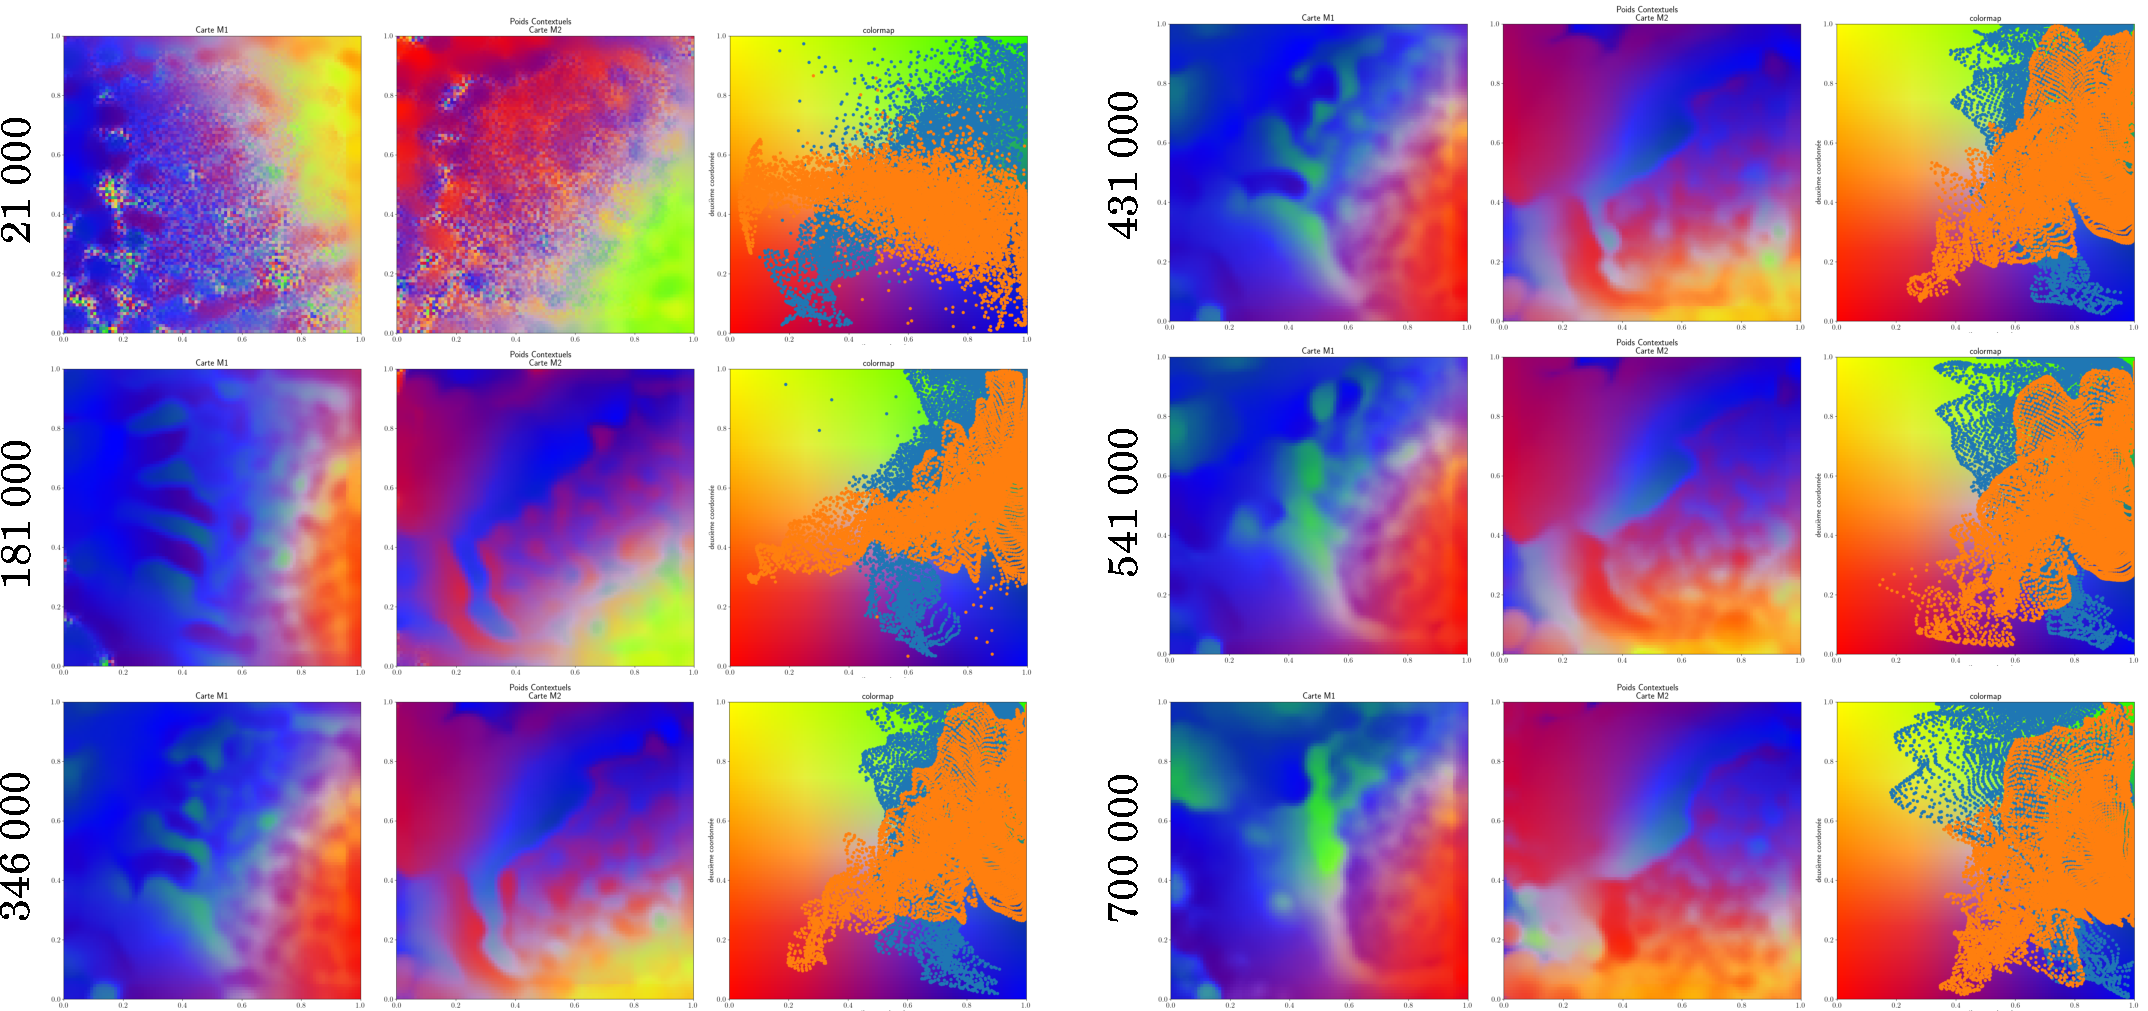
\includegraphics[width=\textwidth]{sphere_rc005_evol_landscape}
	\caption{Evolution des poids contextuels d'une architecture de deux cartes pour $r_c =0.05$. Les points sont représentés sous forme de carte de coloration à gauche et sous forme de disposition dans l'espace des positions sur la figure de droite. On observe une évolution régulière sous forme de motif en hélice, mais cette disposition évolue dans le temps. Après 700000 itérations, la figure semble se déformer vers de nouveaux motifs. Cette organisation ne converge pas. Les valeurs prises par les poids contextuels des cartes $M\m{1}$ (bleu) et $M\m{2}$ (orange) sont tracés sur la carte de coloration, faisant apparaître un motif hélicoïdal évoluant dans le temps.
	\label{fig:rc_005}}
\end{figure}


\begin{figure}
	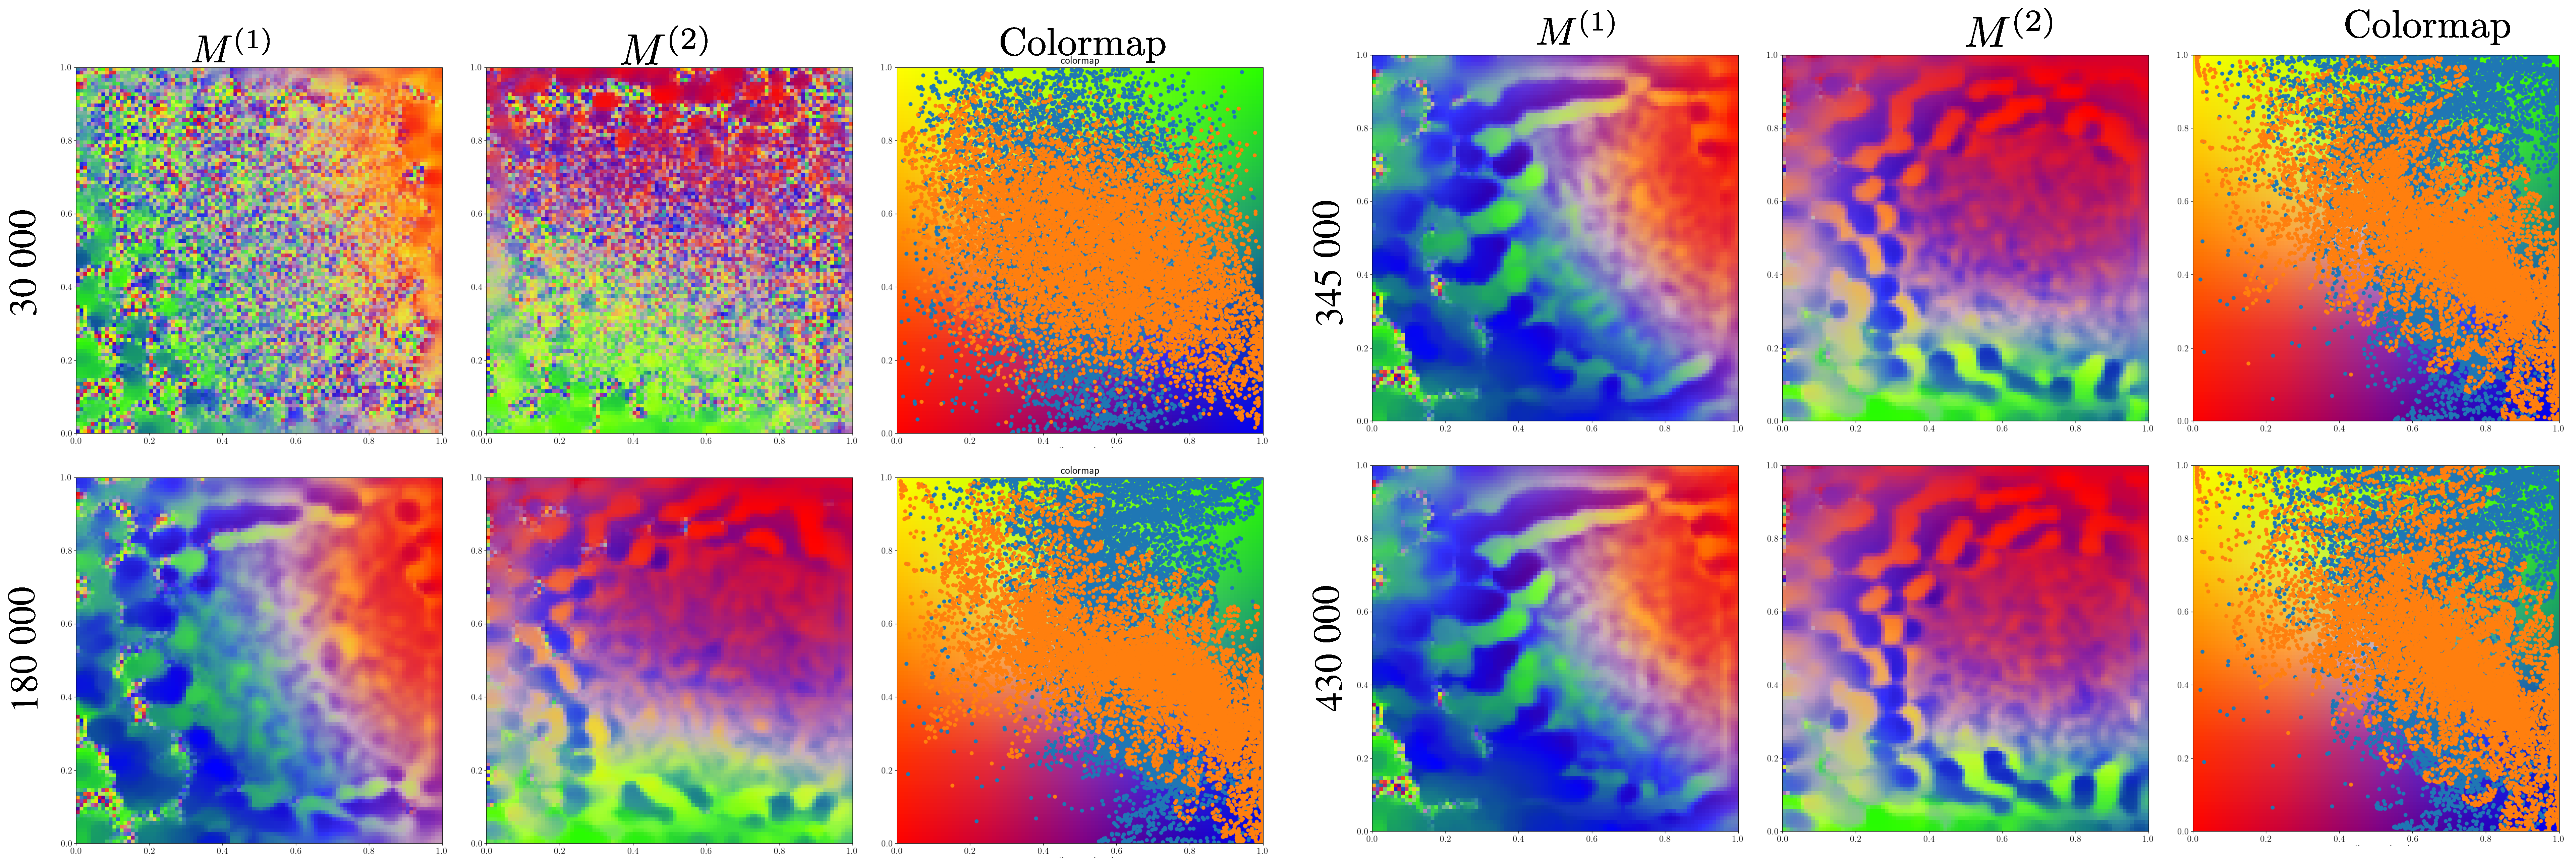
\includegraphics[width=\textwidth]{wc_rc003_evol.pdf}
	\caption{\'Evolution des poids contextuels d'une architecture de deux cartes pour $r_c =0.03$. Les motifs observés sont similaires à ceux observés pour d'autres paramètres. Les poids présentent toujours une forme hélicoïdale évoluant dans le temps.\label{fig:rc_003}}
\end{figure}

\begin{figure}
	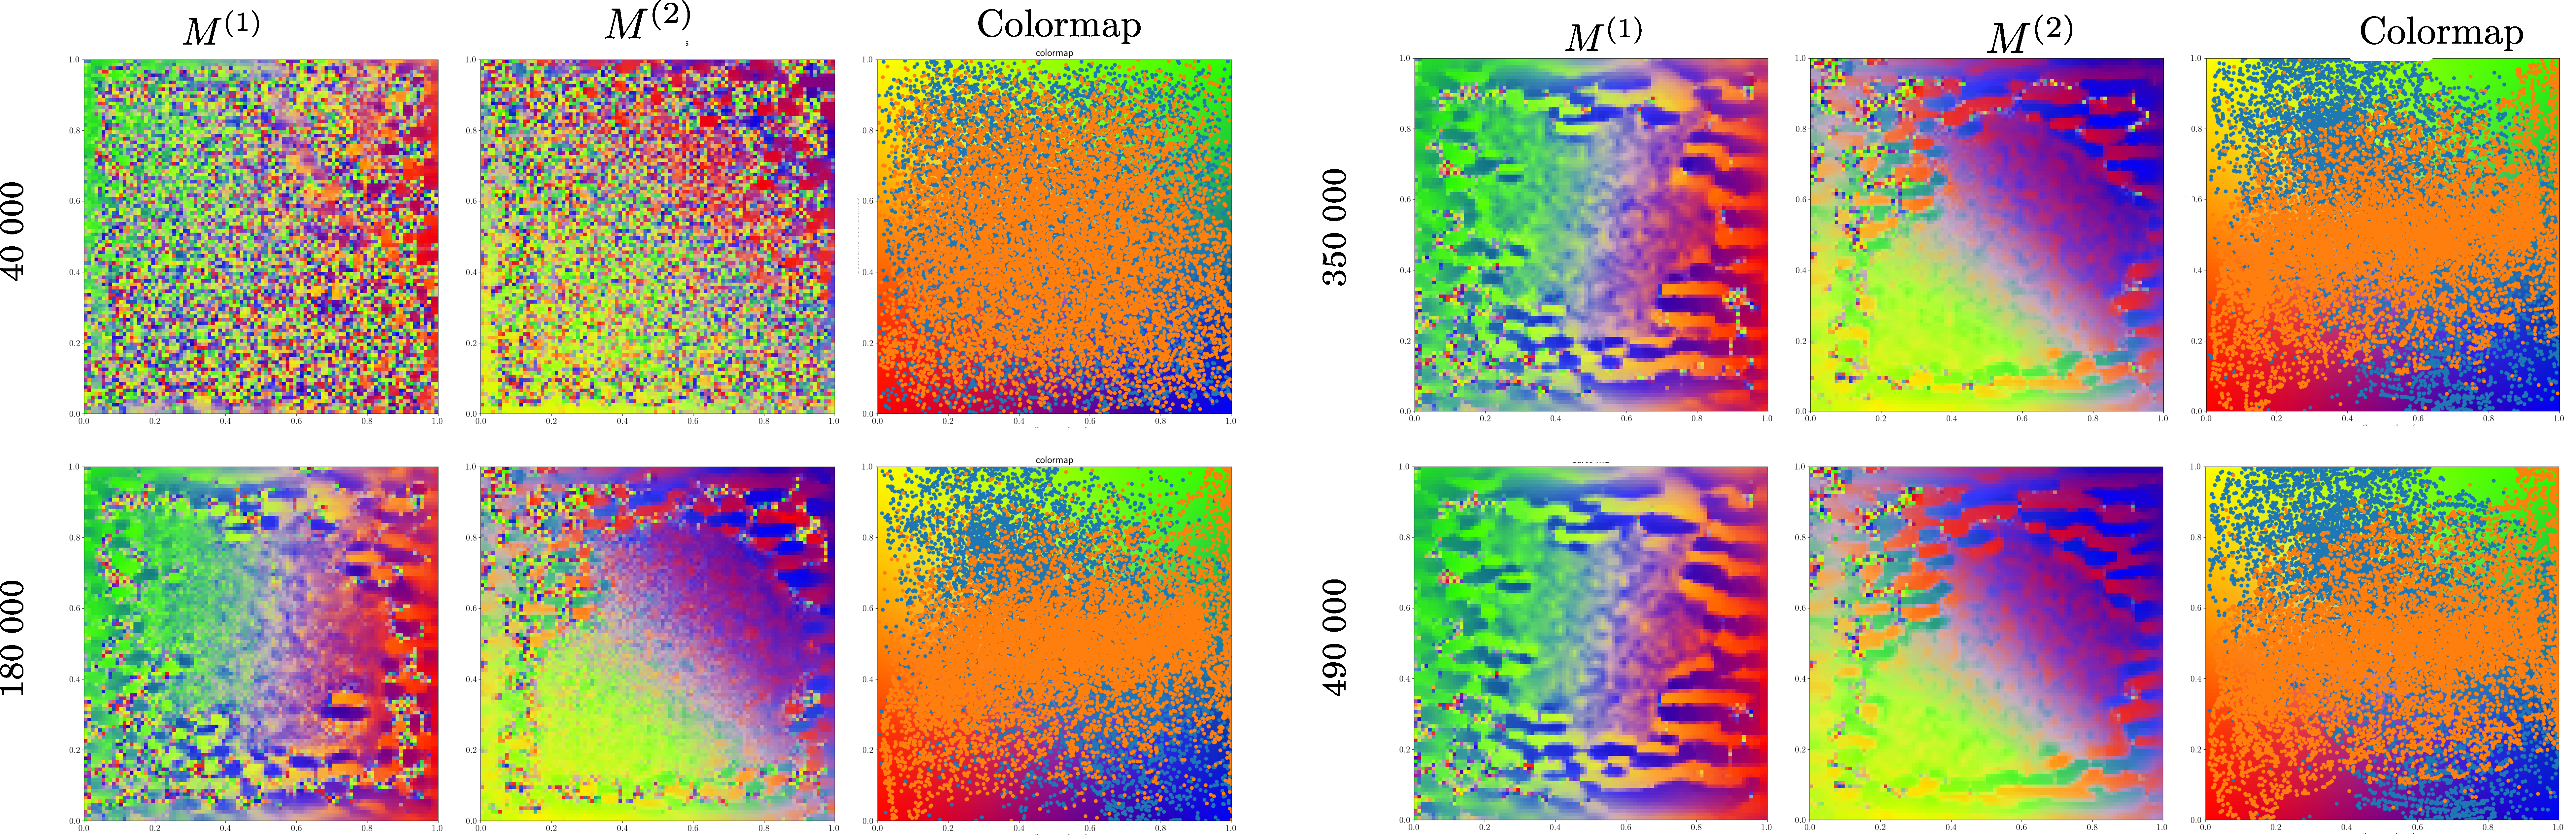
\includegraphics[width=\textwidth]{wc_rc002_evol.pdf}
	\caption{\'Evolution des poids contextuels d'une architecture de deux cartes pour $r_c =0.02$. Les motifs observés sont similaires à ceux observés pour d'autres paramètres. Les poids présentent toujours une forme hélicoïdale évoluant dans le temps. \label{fig:rc_002}}
\end{figure}

\begin{figure}
	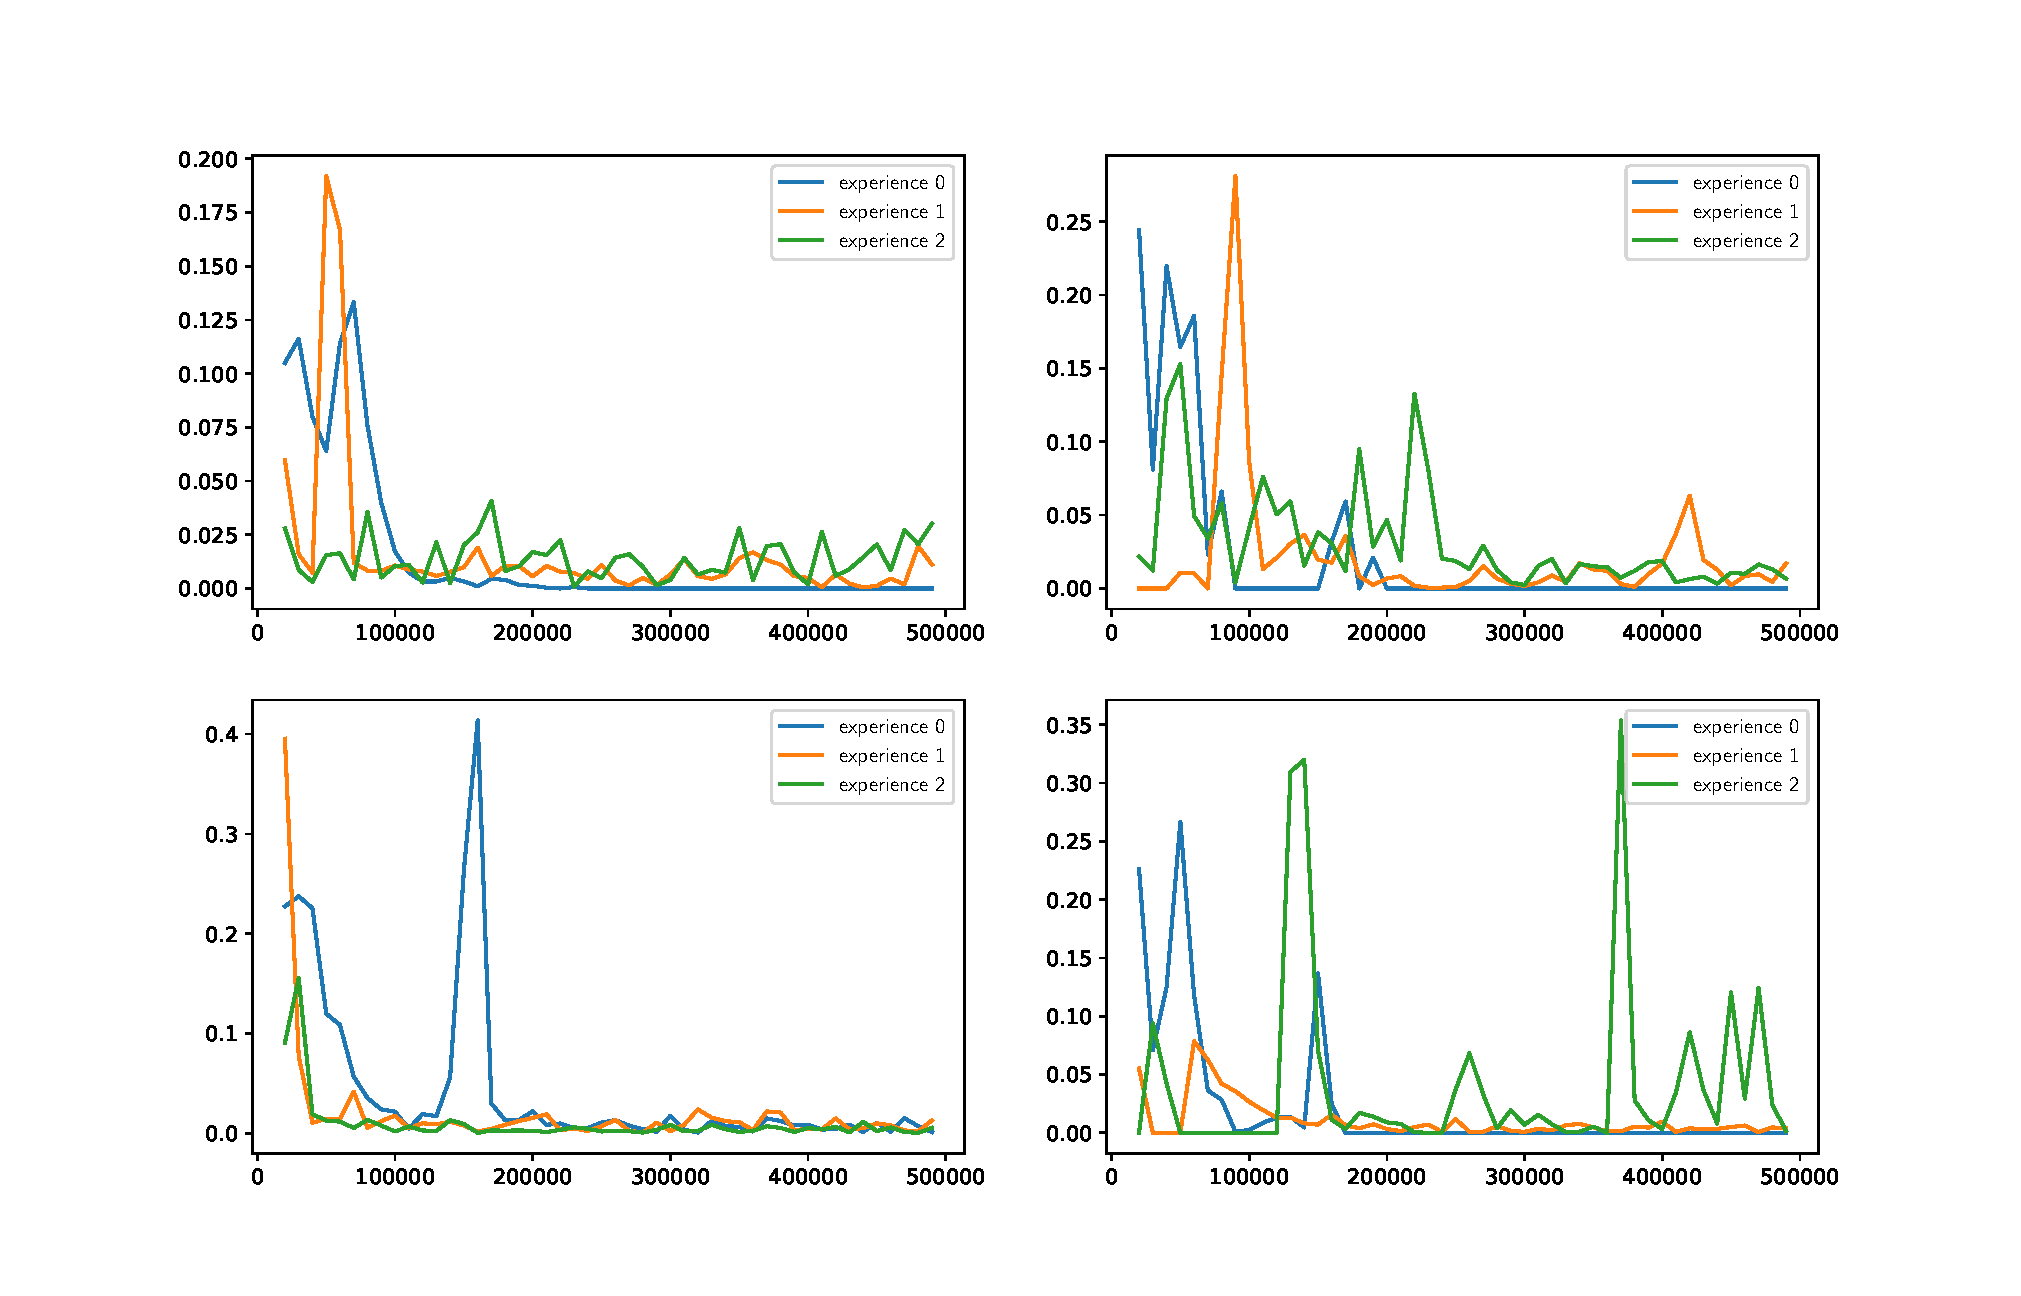
\includegraphics[width=\textwidth]{evol_convergence_poids.pdf}
	\caption{\'Evolution de la différence moyenne entre les poids externes et contextuels au cours de l'apprentissage d'une architecture de 2 cartes sur une sphère 3D en 4 dimensions. Le calcul de différences est réalisé toutes les 10 000 itérations. Nous avons tracé les courbes pour 4 expériences avec $r_e = 0.2$ et $r_c = 0.02$ ainsi que pour les expériences avec $r_e = 0.2$ et $r_c = 0.05$,$r_e = 0.2$ et $r_c = 0.03$. Nous remarquons que cette différence évolue vers une valeur faible, qu'on attend nulle pour une carte stabilisée. Ici les poids tendent vers une valeur faible qui semble stable. Notons que cela ne montre pas forcément la convergence~: les poids peuvent se déplacer faiblement dans une même direction. Le tracé nous assure simplement que l'évolution des poids est lente en fin d'apprentissage. \label{fig:conv_poids}}
\end{figure}

\subsection{Convergence de la relaxation}

Nous nous intéressons ensuite à la convergence de la relaxation sur l'expérience en deux dimensions. Nous avons montré qu'un BMU a du sens dans une carte si la relaxation converge vers un point fixe.
Nous traçons en figure \label{fig:relax} l'évolution du taux de convergence des tests au cours de l'apprentissage pour des structures de deux cartes en deux dimensions, par le
processus décrit au chapitre \ref{chap:relax}. Lors de plusieurs phases de test lancées à des itérations $t$ au cours de l'apprentissage, nous comptons le nombre de pas de relaxation nécessaires à la convergence de la recherche de BMU et traçons sur la figure la moyenne de ce nombre de pas de relaxation à chaque phase $t$. 
Nous traçons également sur la deuxième figure le taux d'échantillons d'un phase de test menant à une convergence de la relaxation. On considère que la relaxation n'a pas convergé si le nombre de pas atteint le seuil maximal de 1000 pas fixé par notre étude. Le nombre de pas de relaxation moyen étant observé de 20 pas, ce seuil est pertinent pour considérer que la relaxation n'a pas convergé.
Nous traçons ces évolutions pour différents paramètres de cartes~: trois expériences de mêmes paramètres $r_e=0.2$ et $r_c = 0.02$ ainsi que les expériences avec $r_c = 0.03$ et $r_c = 0.05$ Dans cette dernière expérience, les poids n'ont pas formé de zones distinctes (voir figure \ref{fig:rc_005_evol}.
Nous voyons que la relaxation converge bien dans entre 95 et 98 \% des cas tout au long de l'apprentissage. Comme dans les cartes 1D, la relaxation converge peu lorsque les poids ne sont pas organisés et le taux de convergence augmente au cours de l'organisation des cartes.
Les valeurs trouvées pour $r_c = 0.05$ sont similaires au cas $r_c = 0.02$, dans lequel les poids ont bien convergé. La relaxation dans des cartes en deux dimensions n'est donc pas liée à la formation de zones stables~: la relaxation trouve un point fixe dans un cas général de cartes en 2D.

Cette observation est prometteuse pour la construction d'architectures. Cela montre que le BMU a un sens dans une carte en deux dimensions.
Nous n'avons pas étudié en deux dimensions l'unicité du BMU en fonction des valeurs d'initialisation de la relaxation.  Nous avons cependant observé que la relaxation converge la plupart du temps, et qu'elle converge vers une valeur dont le poids $\w_e(\bmu)$ est proche de l'entrée externe d'après la faible erreur de quantification vectorielle observée sur les entrées externes en figure \ref{fig:qv2D}.

\begin{figure}
	\centering
	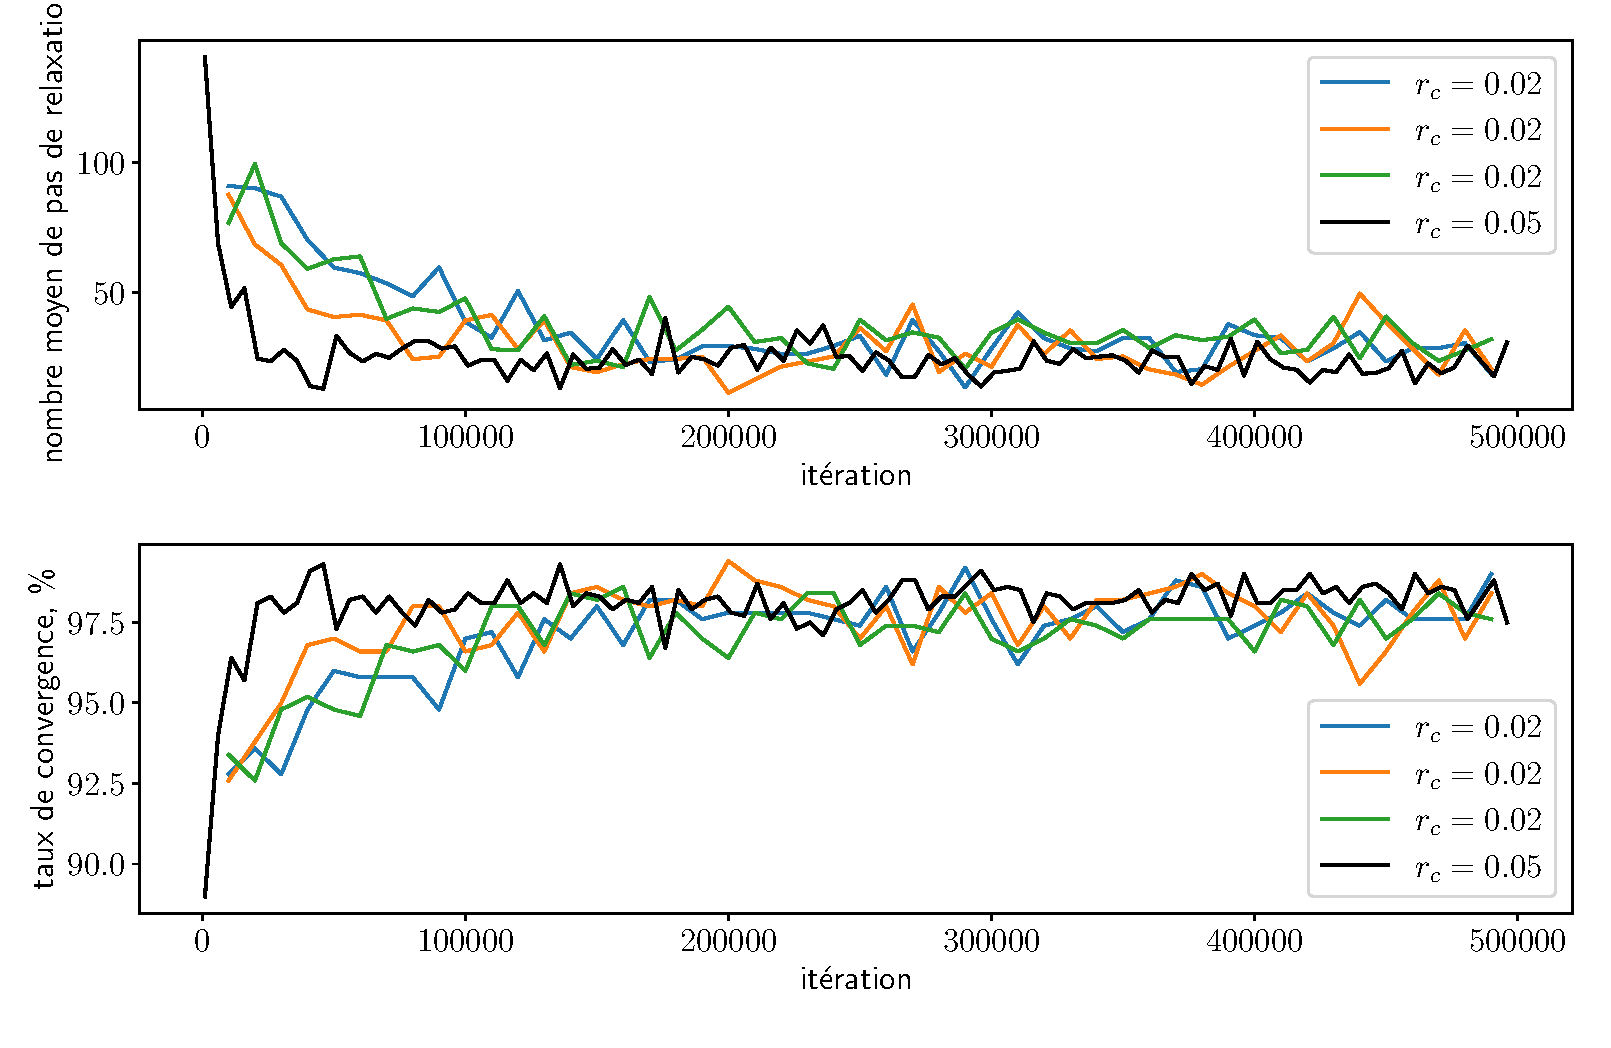
\includegraphics[width=0.7\textwidth]{conv_relax_2maps.pdf}
	\caption{\'Evolution de la convergence de la relaxation au cours de l'apprentissage. Nous avons réalisé les tracés sur trois expériences générées pour $r_c = 0.02$, sur des entrées aléatoires tirées sur la même distribution, une sphère 4D. Pour comparaison, nous traçons également l'évolution pour l'expérience avec $r_c = 0.05$, dans laquelle les poids contextuels n'ont pas convergé. La relaxation converge en fin d'apprentissage~: le BMU a donc un sens dans les cartes en deux dimensions. \label{fig:relax}}
\end{figure}


\subsection{Prédiction d'entrée}

Nous avons vu que les cartes en deux dimensions s'organisent, comme en 1D, de manière à former des zones dans les poids contextuels. 
Nous avons également observé que la recherche de BMU a un sens, car la relaxation converge dans les cartes 2D.
Nous nous attendons donc à ce qu'une architecture de cartes 2D soit en mesure de générer une prédiction.

Pour cela, nous construisons une architecture de trois cartes en deux dimensions. Chaque carte prend en entrée externe une paire de coordonnées d'un espace multimodal en 6D. Ces entrées sont situées sur une sphère de dimension 3 plongée dans l'espace en 6D par le même processus de rotation qu'en 4D. $U$ est donc toujours une variable $2D$. 
Dans cette configuration, la connaissance de deux entrées sur trois et du modèle détermine la troisième~: la prédiction est donc possible.
Nous prenons $r_e = 0.2$ et $r_c = 0.02$, pour des cartes de taille $100 \times 100$. Les cartes sont entraînées sur 250 000 itérations, à l'issue desquelles les poids externes contextuels ont atteint une position stable.

Nous traçons d'abord les poids externes et contextuels des trois cartes sont représentés en Figure~\ref{fig:3som_w}.
L'organisation des poids contextuels conduit à la présence de motifs très semblables à ceux observés sur une architecture de deux cartes.

Nous lançons une étape de prédiction à la fin de l'apprentissage lors de laquelle la carte $M\m{2}$ ne reçoit plus d'entrée externe. 
La valeur de $\w\ext\m{2}(\bmu\m{2})$ est alors utilisée comme prédiction de l'entrée $\inpx\m{2}$.
La Figure~\ref{fig:3som_pred} indique la valeur prédite en fonction de l'entrée $\inpx\m{2}$. 
Les valeurs de $\inpx$ et $\w_e$ étant 2D, nous avons représenté séparément chaque dimension. Cette expérience montre que la prédiction est correctement réalisée, donc que l'architecture a appris le modèle des entrées 2D. 
L'erreur de prédiction observée dans cet exemple est cependant très élevée par rapport à l'échelle de quantification vectorielle de la carte. Ce comportement sera donc à évaluer sur d'autres distributions d'entrée.

\begin{figure}
	\begin{minipage}{\textwidth}
		\centering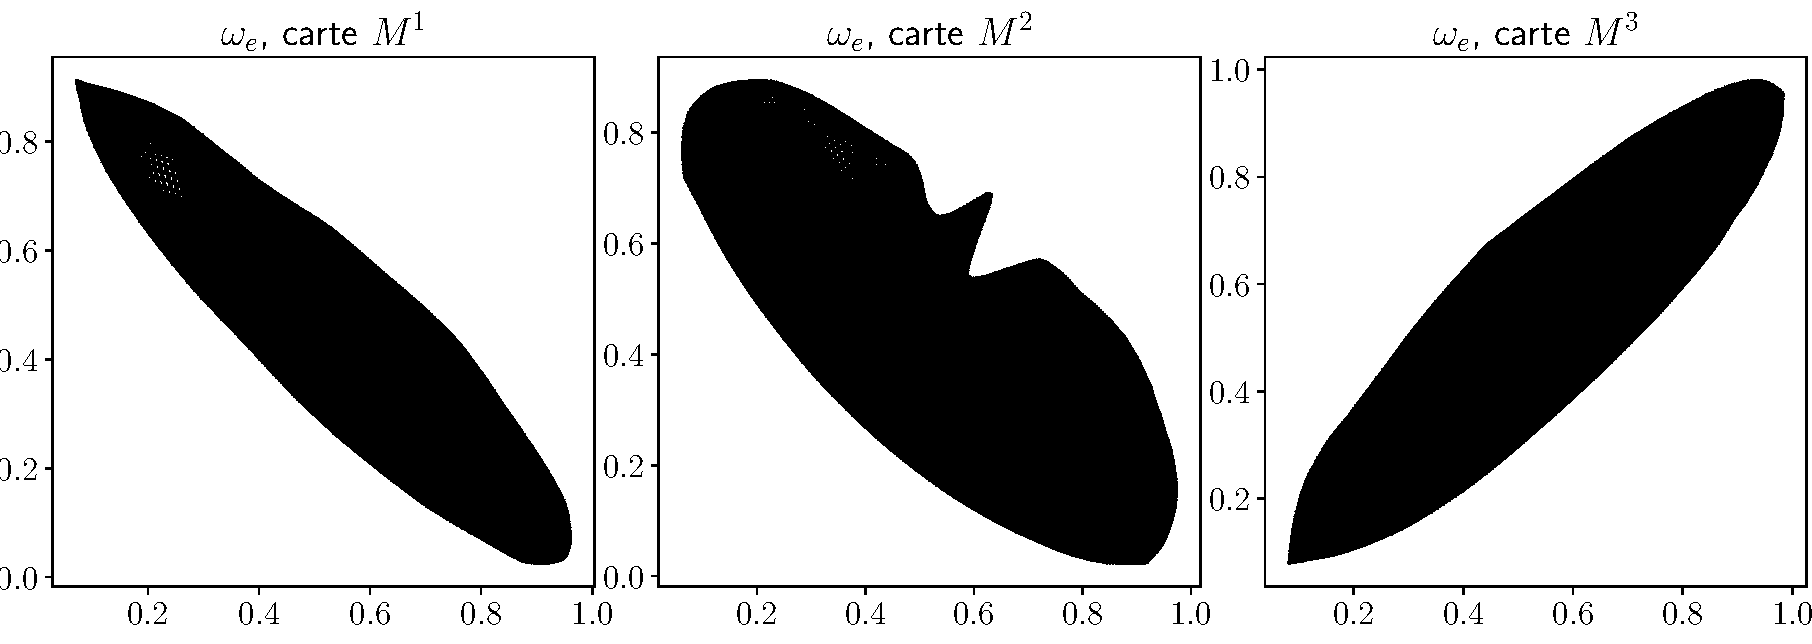
\includegraphics[width=0.7\textwidth]{3SOM_we_rc002.pdf}
	\end{minipage}
	\begin{minipage}{\textwidth}
		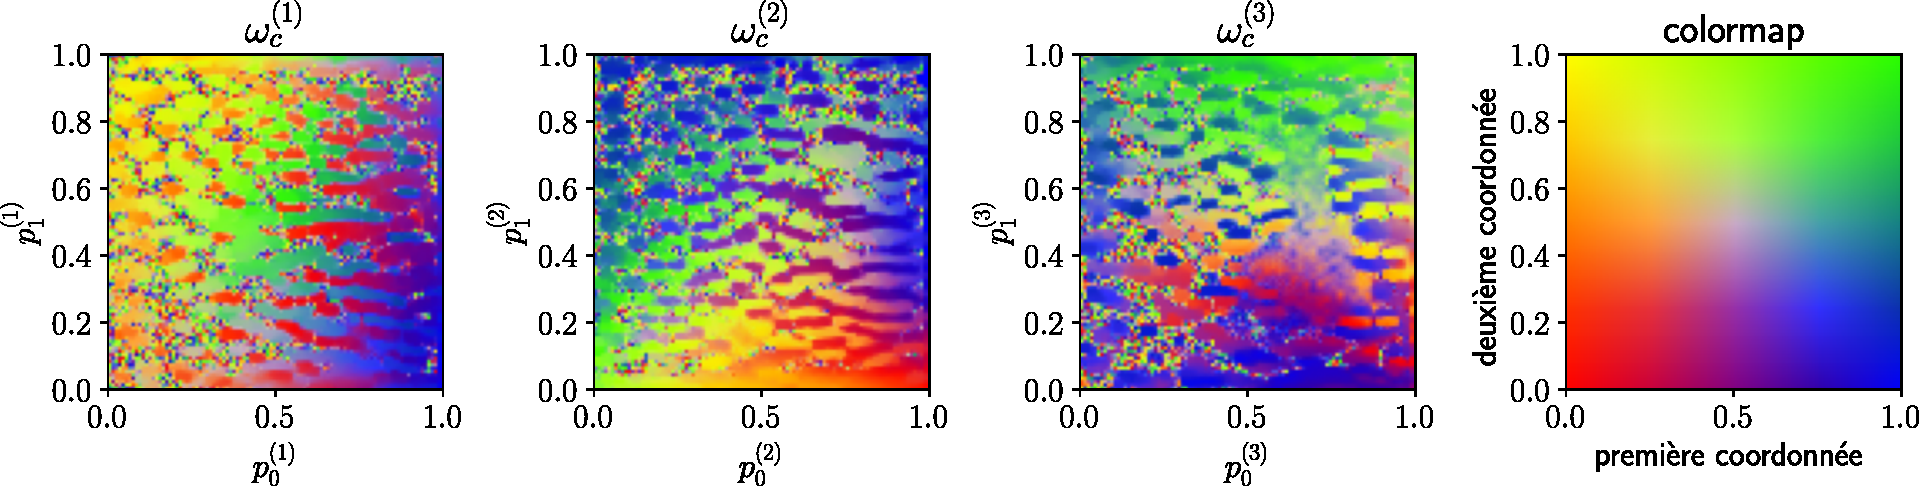
\includegraphics[width=\textwidth]{3SOM_S_wc_239999.pdf}
		\caption{Tracés des poids externes (en haut) dans l'espace des entrées et des poids contextuels (en bas) sous forme de carte de coloration. Les motifs formés par les poids contextuels sont similaires à ceux observés sur deux cartes. \label{fig:3som_w}}
	\end{minipage}
\end{figure}

\begin{figure}
\centering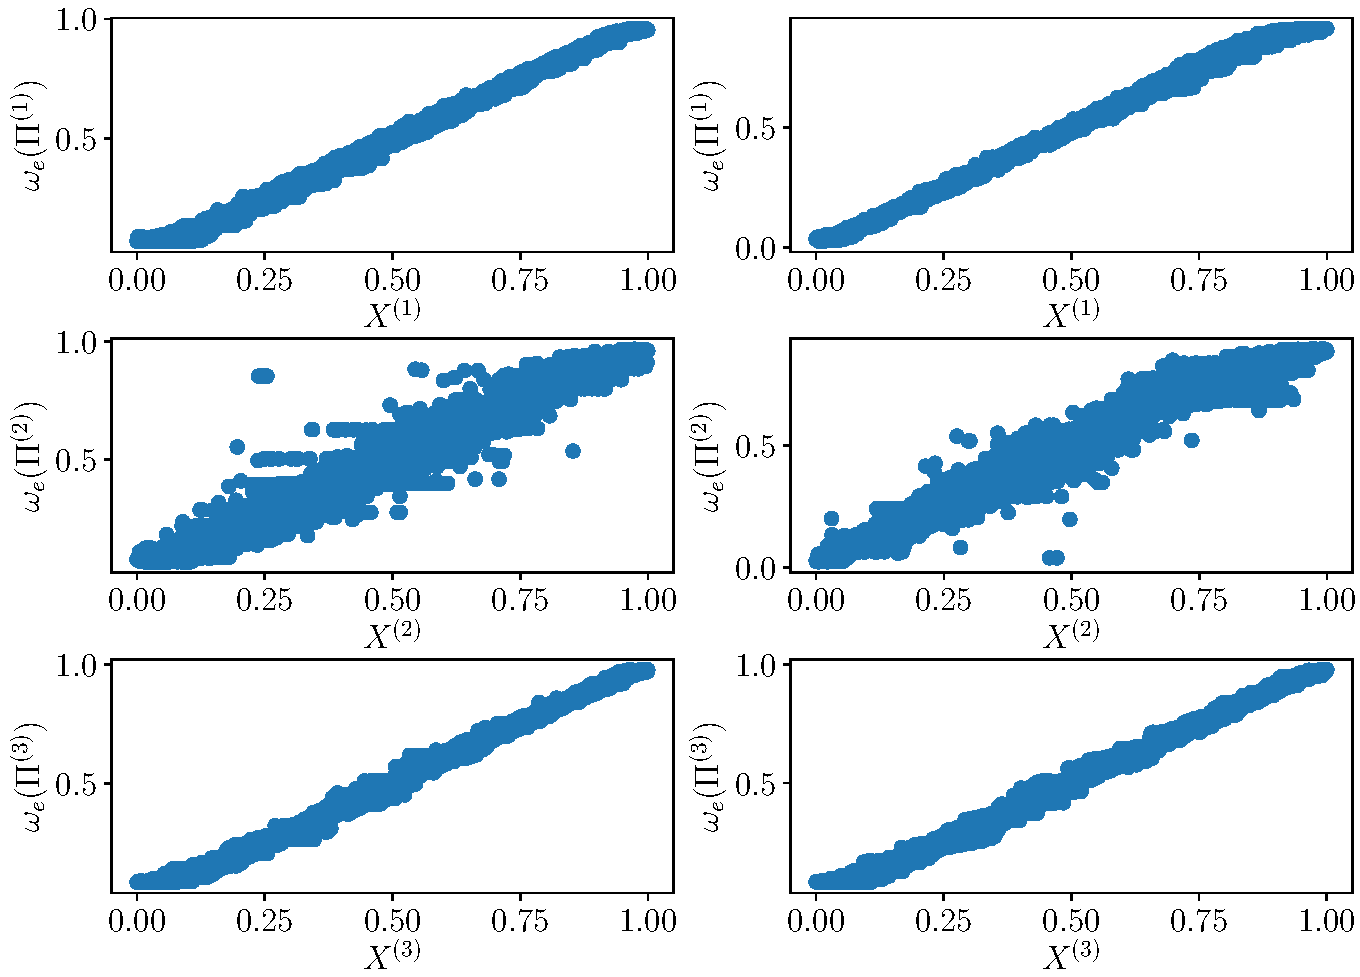
\includegraphics[width=0.7\textwidth]{3som_error_2.pdf}
\caption{Tracé de l'erreur de prédiction $\w_e\m{2}(\bmu\m{2})$ en fonction de la valeur théorique de $X^{(2)}$, non présentée à l'architecture, dans une architecture de trois cartes 2D prenant des entrées $X^{(i)}$ en deux dimensions $[X^{(i)}_0, X^{(i)}_1]$. Nous traçons sur une ligne, pour chaque entrée, les dépendances entre chacune des dimensions.
Lorsque la carte $M^{(2)}$ ne reçoit pas d'entrée externe. Les cartes $M^{(1)}$ et $M^{(3)}$ ayant une activité externe, le graphique montre que la quantification vectorielle est bien réalisée dans ces cartes. La carte $M^{(2)}$ est uniquement activée par les connexions contextuelles venant de $M^{(1)}$ et $M^{(3)}$. La figure du haut montre que la prédiction est correctement réalisée, en observant cependant une erreur très forte. \label{fig:3som_pred}}
\end{figure}

\subsection{Organisation de cartes sur des entrées indépendantes}

Nous nous intéressons enfin à l'organisation d'une architecture de deux cartes prenant des entrées $\inpx\m{1}, \inpx\m{2} \in [0,1]^2 \times 0,1]^2$ indépendantes.
Nous avons également observé la présence de zones distinctes de BMUs lorsque deux cartes apprennent sur des entrées dépendantes. Nous nous plaçons ici dans un cas limite et cherchons à observer si les zones de BMUs sont encore présentes.
Nous prenons des rayons de voisinage $r_e = 0.2, r_c = 0.05$.

Nous nous intéressons ici aux motifs formés par les poids externes et contextuels sur chaque carte.
Les valeurs de ces poids externes et contextuels sont tracés en figure \ref{fig:2som_cub_wc}.
Tracer les poids nous permet ici de comparer l'organisation d'une carte à celle observée en une dimension. Nous soulignons cependant que cette représentation ne permet pas de détecter quelles unités sont effectivement BMU lors d'un test.

Les poids externes sont bien dépliés sur l'ensemble des entrées, ce qui est similaire au cas en une dimension.
Les poids contextuels restent centrés autour de $0.5$~: nous faisons apparaître en bleu et orange sur la carte de coloration les valeurs effectivement prises par les poids contextuels de chaque carte. 
Pourtant, les positions des BMUs de chaque carte observées lors d'un test s'étendent bien sur toute la surface d'une carte. Les poids contextuels auraient dû, pour bien cartographier les positions sur l'autre carte, s'étendre sur tout le carré dans chaque zone.
Ce comportement est à rapprocher du comportement limite observé sur une architecture de 10 cartes en une dimension~: nous avons vu que des architectures de 10 cartes apprenant sur 10 entrées 1D indépendantes voient également leurs poids contextuels se moyenner autour de $0.5$ dans chaque carte.
Proposons une interprétation de ce comportement~: lorsque les entrées présentent une  dépendance, un nombre fini ou un intervalle réduit de valeurs de $\inpx\m{2}$ seront présentées à l'architecture pour une même valeur de $\inpx\m{1}$, correspondant à autant d'entrées contextuelles pour $M\m{1}$. Les poids contextuels situés autour de la position codant pour $\inpx\m{1}$ s'organisent alors comme une carte des valeurs des entrées contextuelles présentées. En une dimension, cette sous carte avait possibilité de s'étendre sur tout l'intervalle de valeurs de $\inpx\m{2}$, formant donc des zones distinctes. En ajoutant des entrées contextuelles, les poids tendaient vers une valeur moyenne des positions, donc 0.5.
En deux dimensions, pour une même valeur de $\inpx\m{1}$, toutes les valeurs possibles de $\inpx\m{2}$ dans le carré $[0,1]^2$ sont présentées. Les poids contextuels n'ont pas la liberté de s'étendre sur toutes ces valeurs et prennent donc une valeur moyenne.

Ce comportement peut apparaître comme une limite de CxSOM car les poids contextuels manquent de liberté pour s'organiser.
Au contraire, nous pouvons aussi envisager ce comportement comme une détection de dépendance entre entrées.
Ce comportement à la limite de CxSOM est une piste de propriété à étudier pour des travaux futurs.

\begin{figure}
	\begin{minipage}{\textwidth}
		\centering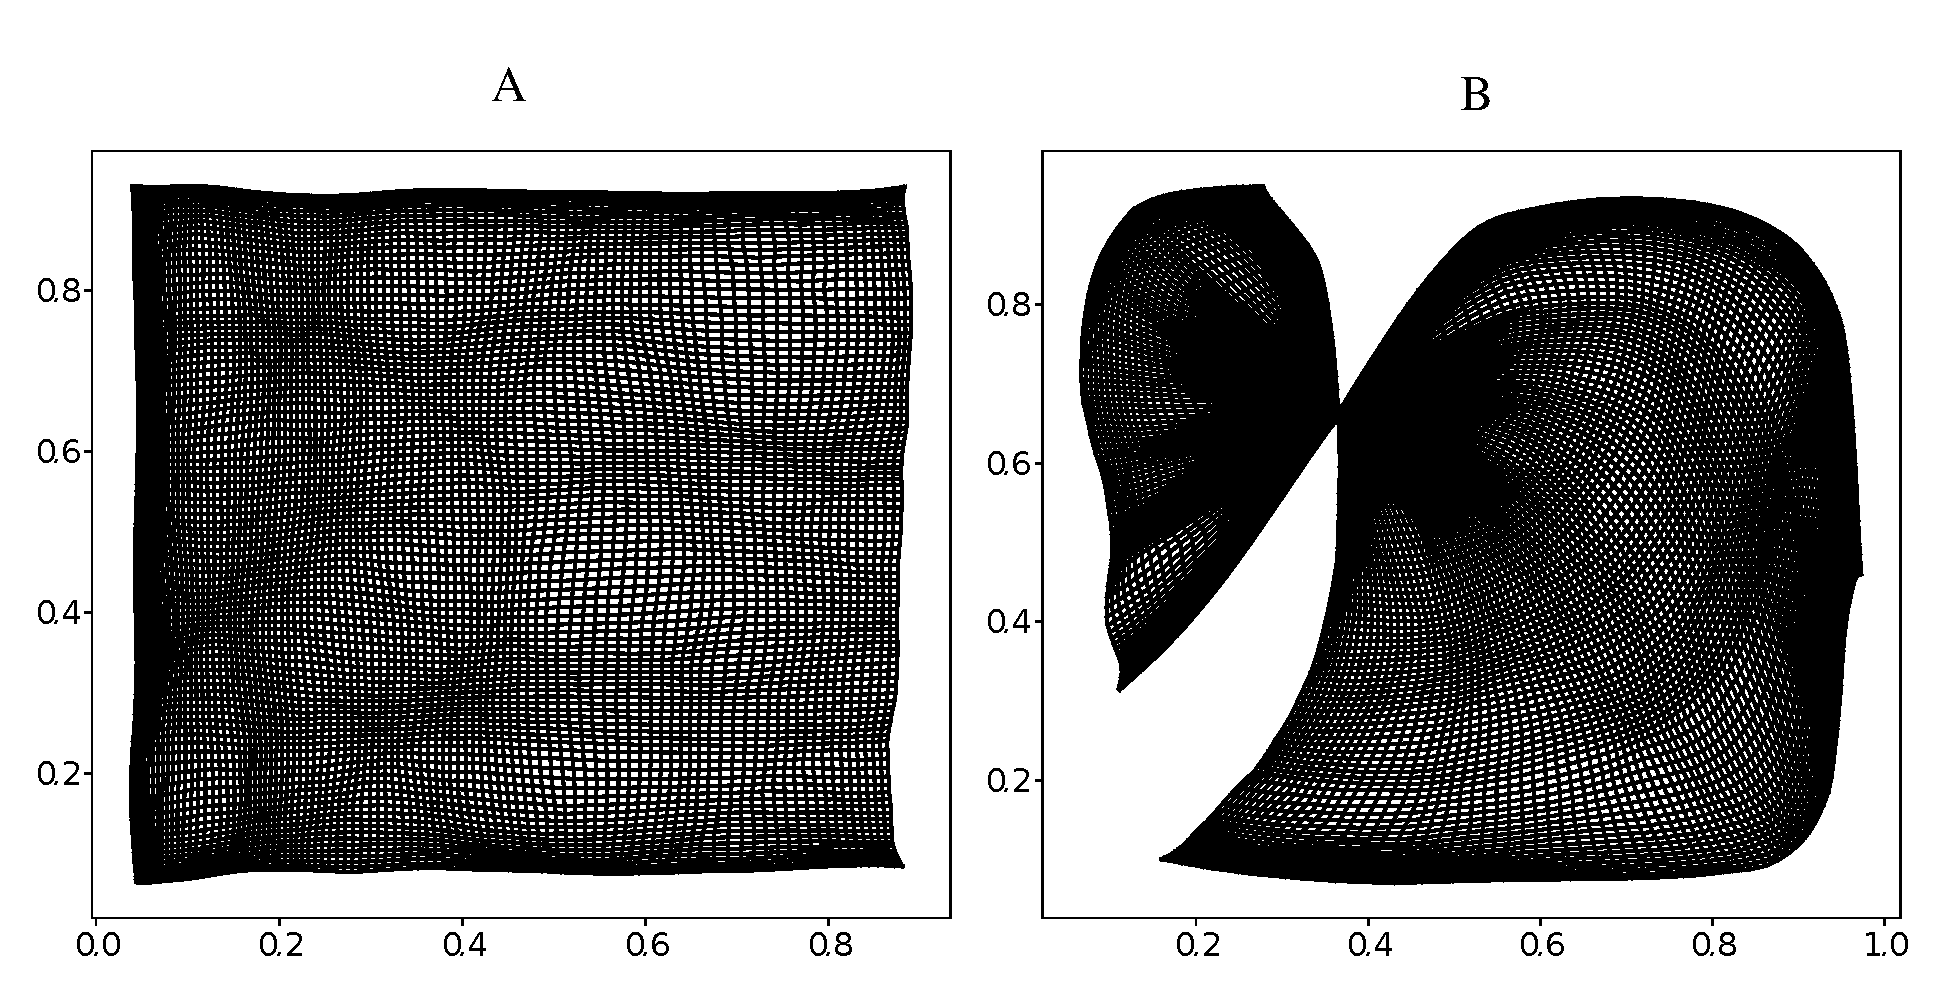
\includegraphics[width=0.6\textwidth]{we_cub_example.pdf}
	\end{minipage}
	\begin{minipage}{\textwidth}
		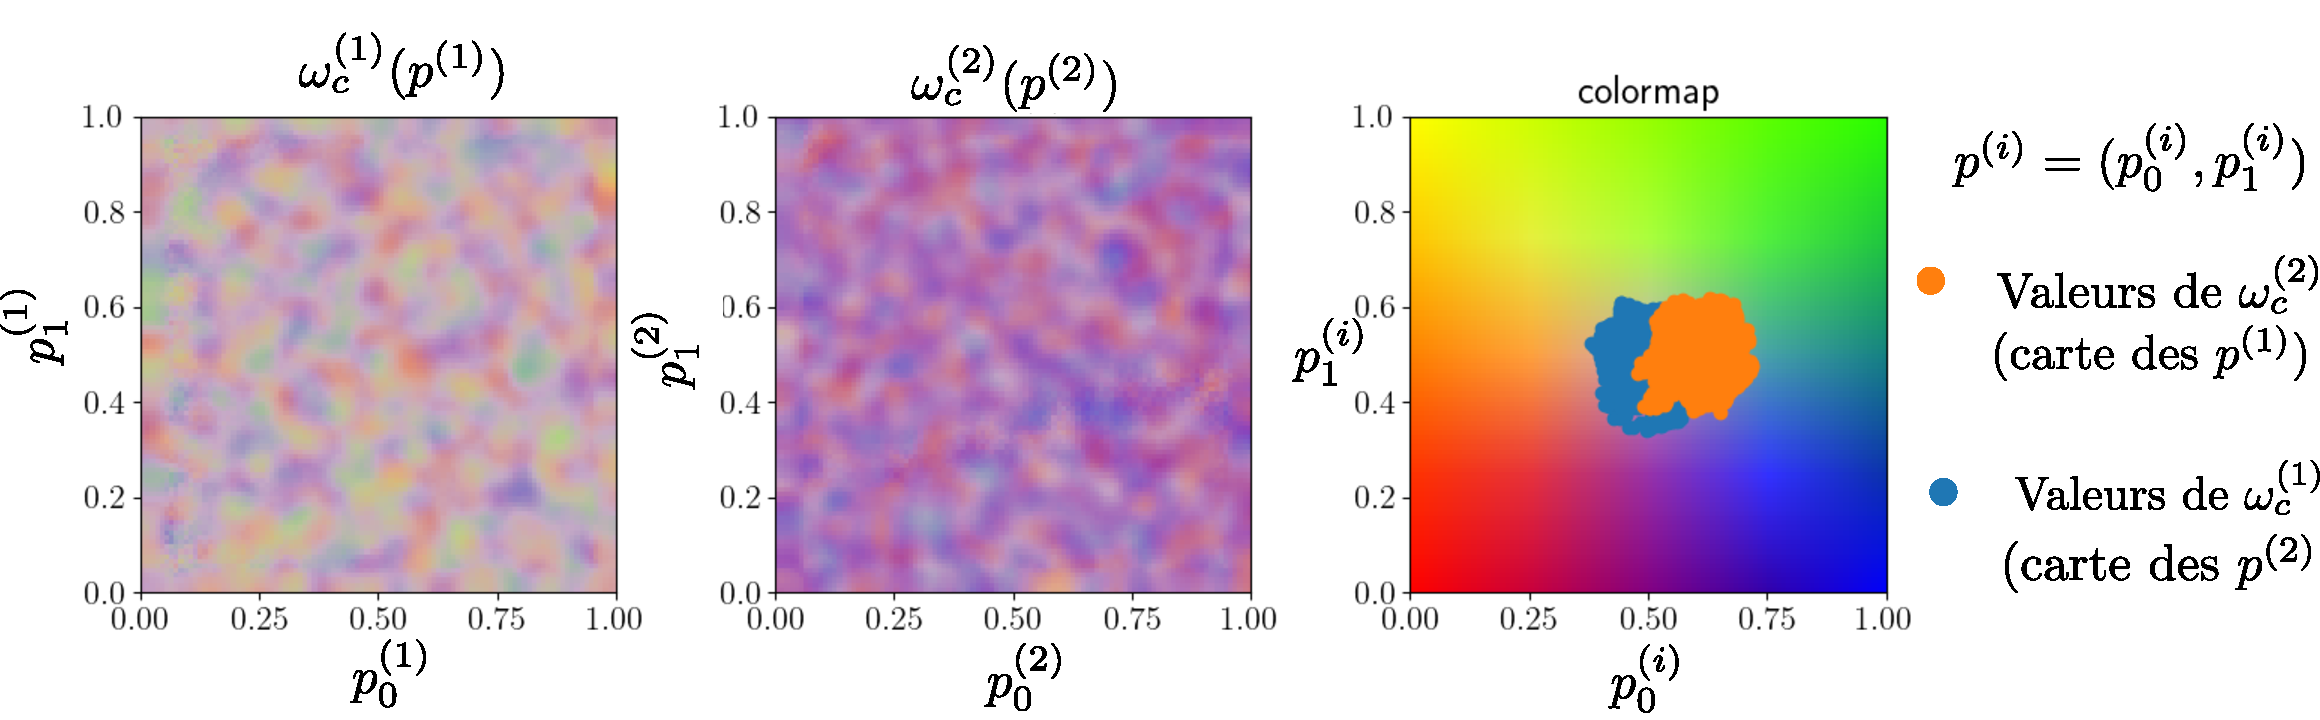
\includegraphics[width=\textwidth]{wc_cub_legend.pdf}
		\caption{En haut: poids externes des cartes $M\m{1}$ et $M\m{2}$ représentés sous forme de distorsion de la carte après 200000 itérations.
	En bas: poids contextuels des cartes pour la même itération, représentés sous forme de carte de couleur en deux dimensions. Un pixel situé à la position $p_i,p_j$ prend comme couleur correspondante la valeur 2D de son poids contextuel, associé à une couleur par la carte de coloration représentée à droite de la figure.
	Les points orange et bleus indiqués sur la carte de coloration sont les valeurs effectivement prises par toutes les valeurs de $\w_c^{(1)}$ et $\w_c^{(2)}$, cartographiant les positions des BMUs de l'autre carte.
	On remarque donc que les poids contextuels ne se déplient pas sur toutes les valeurs prises par les BMUS, car toutes les unités de la carte ont été BMU lors de cette phase de test.\label{fig:2som_cub_wc}}
	\end{minipage}
\end{figure}


\section{Conclusion}

Les expériences proposées dans ce chapitre sur les cartes en deux dimensions donnent une idée des comportements auxquels on peut s'attendre dans un cas plus général d'architecture.
Ces expériences nous ont également permis de vérifier la méthode d'étude de carte construite tout au long de cette thèse et constituent une première application des indicateurs proposés au chapitre précédent.
Nous avons d'abord observé que l'émergence de zones de poids contextuels est une propriété qui se transpose sur des cartes en deux dimensions. Ces zones constituent donc un point clé des architectures CxSOM.
La formation de ces zones permet, comme sur des cartes 1D, de séparer les valeurs de $U$ en fonction des positions des BMUs et $U$ est une fonction du BMU dans chacune des cartes en deux dimensions également.
Cette séparation est correctement évaluée par le ratio de corrélation.
La convergence des poids, contrairement aux cartes en une dimension, n'est pas assurée en fonction des paramètres d'apprentissage et constitue un point à analyser lors de la construction d'architectures de cartes en deux dimensions. 
Par ailleurs, nous avons déplié les poids externes lors d'une étape d'initialisation afin de s'assurer que la carte 2D ne présente pas de "point de torsion". La robustesse de l'algorithme CxSOM sur des cartes "mal organisées" est un point à étudier avant une éventuelle application de l'algorithme.


Nous remarquons que la forme des motifs spatiaux formés par les poids contextuels sont plus variés que dans le cas des cartes en une dimension~; il serait intéressant d'explorer la formation de ces motifs sur d'autres dispositions d'entrées. Ces motifs rappellent ceux émergeant d'autre processus d'organisation, tels que les motifs de Turing. Ces motifs émergent de processus de diffusion, ce qui n'est a priori pas le cas sur les cartes de Kohonen~: l'organisation des cartes est guidée par la présentation d'une séquence aléatoire d'entrées. Il est cependant intéressant d'observer la similarité existant dans les motifs, qui montrent que l'organisation des cartes est issue d'une dynamique complexe (au sens des systèmes complexes).
Les poids contextuels montrent également l'émergence de motifs temporels lors de l'apprentissage~: l'organisation en hélice pour $r_c = 0.05$. Ces observations montrent que les mécanismes d'apprentissage émergeant dans des cartes en deux dimensions sont plus complexes qu'en une dimension. Cela peut être un atout pour le modèle car cela laisse la porte ouverte à des comportements plus complexes sur des cartes 2D~; mais cela apporte plus de difficulté pour une éventuelle compréhension du modèle.
Ainsi, il est pertinent d'étudier l'organisation des cartes d'un point de vue macroscopique pour la suite des travaux. Si la forme des motifs en 1D nous apportait une compréhension du comportement d'une architecture de trois cartes, il est compliqué de prédire l'apprentissage d'une architecture de cartes 2D et de plus nombreuses cartes à partir de la forme des poids.


\begin{figure}
\centering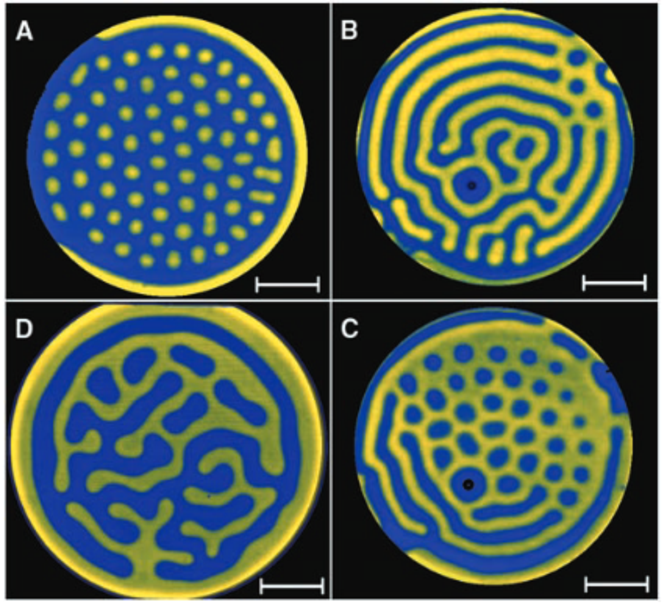
\includegraphics[width=0.5\textwidth]{turing_pattern_chem.pdf}
\caption{Motifs de Turing observés lors d'une réaction de diffusion chimique. Ces motifs émergent après l'introduction d'une perturbation dans un système initialement stable. Les différents motifs A,B,C,D sont des états atteint dans différentes expériences en fonction des paramètres de la réaction. Dans nos cartes, nous observons des motifs similaires au motif A lorsque $r_c = 0.02$, mais nous observons également des motifs rappelant C et D pour des rayons de voisinage différents. Notons cependant que l'organisation des cartes n'est a priori pas un processus de diffusion et est générée par la présentation d'une séquence d'entrées.  \label{fig:turing}}
\end{figure}




\ifSubfilesClassLoaded{
    \printbibliography
    %\externaldocument{../main.tex}   
}{}
\end{document}



% PLAN


% Convergence des poids :
% - Dépend des paramètres, contrairement à la carte en 1D on n'arrive pas forcément dans une position stable
% - Rc = 0.02 : point fixe, avec une partie 
% - Chaque expérience différente : grande dépendance aux conditions initiales. 